\title{Extrapolating expected accuracies for multi-class classification}
\author{Charles Zheng, Rakesh Achanta and Yuval Benjamini}
\date{\today}

\documentclass[12pt]{article} 

% packages with special commands
\usepackage{amssymb, amsmath}
\usepackage{epsfig}
\usepackage{array}
\usepackage{ifthen}
\usepackage{color}
\usepackage{fancyhdr}
\usepackage{graphicx}
\usepackage{mathtools}
\usepackage{csquotes}
\usepackage{multirow}
\usepackage{xcolor}
\usepackage{chngcntr}
\usepackage{apptools}
\AtAppendix{\counterwithin{lemma}{section}}

\newcommand\crule[3][black]{\textcolor{#1}{\rule{#2}{#3}}}

\definecolor{grey}{rgb}{0.5,0.5,0.5}
\definecolor{color1}{RGB}{128,13,13}
\definecolor{color2}{RGB}{70,128,13}
\definecolor{color3}{RGB}{13,128,128}
\definecolor{color4}{RGB}{70,13,128}

\begin{document}
\maketitle

\newcommand{\skone}{\mathcal{S}_{k_1}}
\newcommand{\sktwo}{\mathcal{S}_{k_2}}

\newcommand{\tr}{\text{tr}}
\newcommand{\E}{\textbf{E}}
\newcommand{\diag}{\text{diag}}
\newcommand{\argmax}{\text{argmax}}
\newcommand{\Cov}{\text{Cov}}
\newcommand{\Var}{\text{Var}}
\newcommand{\argmin}{\text{argmin}}
\newcommand{\Vol}{\text{Vol}}
\newcommand{\comm}[1]{}
\newcommand{\indep}{\rotatebox[origin=c]{90}{$\models$}}
\newcommand{\Cor}{\text{Cor}}
\newtheorem{theorem}{Theorem}[section]
\newtheorem{proposition}{Proposition}[section]
\newtheorem{corollary}{Corollary}[theorem]
\newtheorem{lemma}{Lemma}[section]
\newtheorem{definition}{Definition}[section]
\newcommand{\bZ}{\boldsymbol{Z}}
\newcommand{\bz}{\boldsymbol{z}}
\newcommand{\bx}{\boldsymbol{x}}
\newcommand{\bX}{\boldsymbol{X}}

\newcommand{\bH}{\boldsymbol{H}}


\begin{abstract}
The difficulty of multi-class classification generally increases with
the number of classes.  Using data from a subset of the classes, can
we predict how well a classifier will scale with an increased number
of classes?  Under the assumption that the classes are sampled
exchangeably, and under the assumption that the classifier is
generative (e.g. QDA or Naive Bayes), we show that the expected
accuracy when the classifier is trained on $k$ classes is the $k-1$st
moment of a \emph{conditional accuracy distribution}, which can be
estimated from data.  This provides the theoretical foundation for
performance extrapolation based on pseudolikelihood, unbiased
estimation, and high-dimensional asymptotics.  We investigate the
robustness of our methods to non-generative classifiers in simulations
and one optical character recognition example.
\end{abstract}

\section{Introduction}
An algorithm that can use sensory information to automatically
 distinguish between multiple scenarios has increasingly many applications
 in modern life. Examples include detecting the speaker from his voice patterns, 
identifying the author from her written text, or labeling the object 
category from its image. All these examples can be described as multi-class classification problems:
the algorithm observes an input $x$, and uses the classifier function $f$ to guess
the label $y$ from a discrete set $\mathcal{Y}$ of possible labels. 
In all applications described above, the space of potential labels is practically infinite.
But in any particular experiment, the number of different labels $k$ used would be finite.
A natural question, then, is how changing the number of 
possible labels affects the classification accuracy. 

More technically, we consider a sequence of classification
problems on finite label subsets
$\mathcal{S}_1 \subset \cdots \subset \mathcal{S}_K \subset \mathcal{Y}$,
where in the $i$-th problem, one constructs the classification rule
$f^{(i)}:\mathcal{X} \to \mathcal{S}_i$.  Supposing that $(X, Y)$ have
a joint distribution, define the misclassification error for the
$i$-th problem as
\[
\text{Err}^{(i)} = \Pr[f^{(i)}(X) \neq Y|Y \in \mathcal{S}_i].
\]
The problem of \emph{performance extrapolation} is the following: using data
from only $\mathcal{S}_k$, can one predict the misclassification error
 on the larger label set $\mathcal{S}_K$, with $K> k$?
Note that unlike other
extrapolations from a smaller sample to a larger population, 
the classification problem becomes harder as the number of distractor classes
increases. 

Accurate answers to this 
problem are not only of theoretical interest, but also have practical implications:
\begin{itemize} 
\item Example 1: A researcher develops a classifier for the purpose of labelling
images in 10,000 classes. However, for a pilot study, her resources are sufficient to 
tag only a smaller subset of these classes, perhaps 100. Can she estimate how well the algorithm 
work on the full set of classes based on an initial "pilot" subsample of class labels?
\item Example 2: A neuroscientist is interested in how well the brain activity 
in various regions of the brain can discriminate between different classes of stimuli.
Kay et al. [1] obtained fMRI brain scans which record how a single
subject's visual cortex responds to natural images. They wanted to know how 
well the brain signals could discriminate between different images. For a set of 1750
photographs, they constructed a classifier which
achieved over 0.75 accuracy of classification. Based on
exponential extrapolation, they estimate that it would take on the
order of $10^{9.5}$ classes before the accuracy of the model drops
below 0.10!  A theory of performance extrapolation could be useful for
the purpose of making such extrapolations in a more principled way.
\item The stories just described can be viewed as a metaphor for typical
paradigm of machine learning research, where academic researchers,
working under limited resources, develop novel algorithms and apply
them to relatively small-scale datasets. Those same algorithms may
then be adopted by companies and applied to much larger datasets with
many more classes. In this scenario, it would be convenient if one
could simply assume that performance on the smaller-scale
classification problems was highly representative of performance on
larger-scale problems. 
\end{itemize}

Previous works have shown that generalizing from a small set of classes 
to a larger one is not straightforward. In a paper titled ``What
does classifying more than 10,000 Image Categories Tell Us,'' Deng and
co-authors compared the performance of four different classifiers on
three different scales: a small-scale (1,000-class) problem,
medium-scale (7,404-class) problem, and large-scale (10,184-class)
problem (all from ImageNet.)  They found that while the
nearest-neighbor classifier outperformed the support vector machine
classifier (SVM) in the small and medium scale, the ranking switched
in the large scale, where the SVM classifier outperformed
nearest-neighbor.  As they write in their conclusion, ``we cannot
always rely on experiments on small datasets to predict performance at
large scale.'' Theory for performance
extrapolation may therefore reveal models with bad scaling properties in the
pilot stages of development.

Our primary goal in this paper is to formulate this question, and
identify scenarios where answers are possible. 
The most important condition is that the smaller problem would be 
representative of the larger one. For simplicity, we
assume that in both $\mathcal{S}_K$ and $\mathcal{S}_k$ are iid samples
from a population (or distribution) of labels. (Other sampling 
mechanisms would require some modification). 
The condition of i.i.d. sampling of labels ensures that the
separation of labels in a random set $\mathcal{S}_K$ can be inferred by
looking at the empirical separation in $\mathcal{S}_k$, and
therefore that some estimate of the achievable accuracy on
$\mathcal{S}_K$ can be obtained.

Our analysis considers a restricted set of classifiers,
\emph{marginal classifiers}, which train a separate model for each class. 
This convenient property allows us to
characterize the accuracy of the classifier by selectively
conditioning on one class at a time.  In section \ref{sec:extrapolation}, we use this
technique to reveal that the expected risk for classifying on the
label set $\mathcal{Y}_k$, for all $k$, is governed by a
specific function - the \emph{conditional risk} -  
that depends on the true distributions and the classifier. 
As long as one can recover the conditional risk
function $\bar{D}(u)$, one can compute the average risk for any number
of classes. 
  In section 5, we
empirically study the performance curves of classifiers on sequences
of classification tasks.  Since marginal classifiers only comprise a
minority of the classifiers used in practice, we applied our methods
to a variety of marginal and non-marginal classifiers in
simulations and in one OCR dataset.  Our methods have varying success
on marginal and non-marginal classifiers, but seem to work badly
for neural networks.
\newline

\noindent\emph{Our contribution.}

To our knowledge, we are the first to formalize the problem of
prediction extrapolation.  We develop a general theory for prediction
extrapolation under \emph{general class priors} and under bounded cost
functions.  [[TODO: mention estimation results, theory]]


% semantic distance is not explained

%The hierarchy of labels is often represented by a tree $T$, where the
%vertices $V$ are the set of labels, and the edges indicate
%superclass-subclass relationships.  One of the earlier examples is
%Chakrabarti (1998), who classified online texts into topic taxonomies.
%One of the taxonomies, reprinted from their paper, is shown in
%Figure \ref{fig:chakra}.
% sometimes the classes are only the leaves, and sometimes all nodes are classes

%\begin{figure}[h]
%\centering
%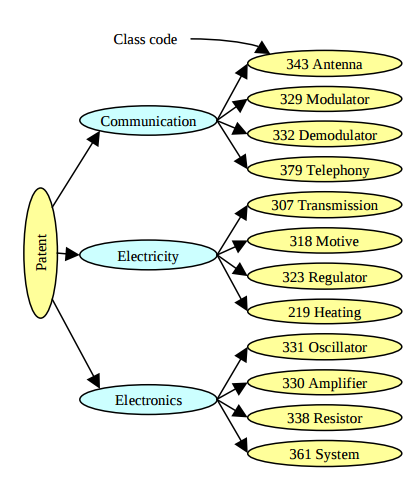
\includegraphics[scale = 0.4]{chakrabarti_1998.png}
%\caption{A topic taxonomy reprinted from Chakrabarti (1998)}\label{fig:chakra}
%\end{figure}

%Cost functions for hierarchical class function are commonly derived
%from graph distances induced by the tree $T$.  For example, one might
%define $C(y', y)$ to be the \emph{graph distance} between $y$ and
%$y'$--that is, the minimal number of edges in the graph for any path
%between $y$ and $y'$.

%[examples of multi-class classifiers? LDA, QDA, OVA, OVO?]

\section{Framework}\label{sec:formulation}

\subsection{Problem Formulation}

%Let $\mathcal{Y}$ be a collection of labels and $\mathcal{X}$ be a
%space of feature vectors.  

%The joint distribution of a pair 
%$(x,y)\in (\mathcal{X},\mathcal{Y})$ can be factored into a prior on the labels
%$\pi_y$ and a conditional distribution on the examples for that label 
%that are represented by feature vectors $x\sim F_y$ supported on $\mathcal{X}$.
%For each experiment, the prior is concentrated on a discrete set of distinct labels
%$\mathcal{S}_y={\y_1,...,\y_k}$. We assume for now that the prior is uniform on $\mathcal{S}$.
%labels. , represetfeature vectors For each label $y \in \mathcal{Y}$, there
%exists a distribution $F_y$ supported on $\mathcal{X}$.  Also suppose
%that there exists a \emph{cost function} $C(\hat{y}, y)$ which
%measures the cost of incorrectly labelling an instance as $\hat{y}$
%when the correct label is $y$. For now, we will consider the $0-1$ cost
%where $C(\hat{y},y)=0$ if $\hat{y}=y$ and 1 for any $\hat{y}\neq y$. 

%The performance of a classification rule on a problem is evaluated by
%specifying a \emph{cost function.}  If the true class is $y$, but the
%classifier outputs $y'$, the severity of this misclassification is
%quantified by $C(y', y)$.  The most common cost function
%is \emph{zero-one loss}: the cost is zero for correct classifications,
%and the cost is one for all incorrect classifications, i.e. $C(y', y)
%= \delta_{y}(y').$


\begin{figure}[h]
\centering
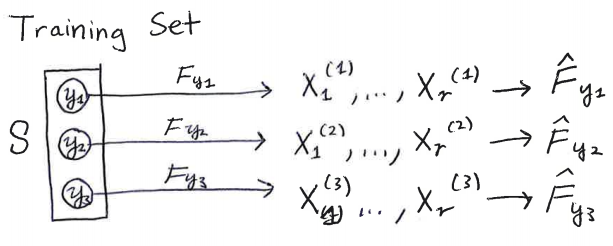
\includegraphics[scale = 0.4]{extrapolation_figures/training_set.png}
\caption{Training set}\label{fig:training_set}
\end{figure}

\begin{figure}[h]
\centering
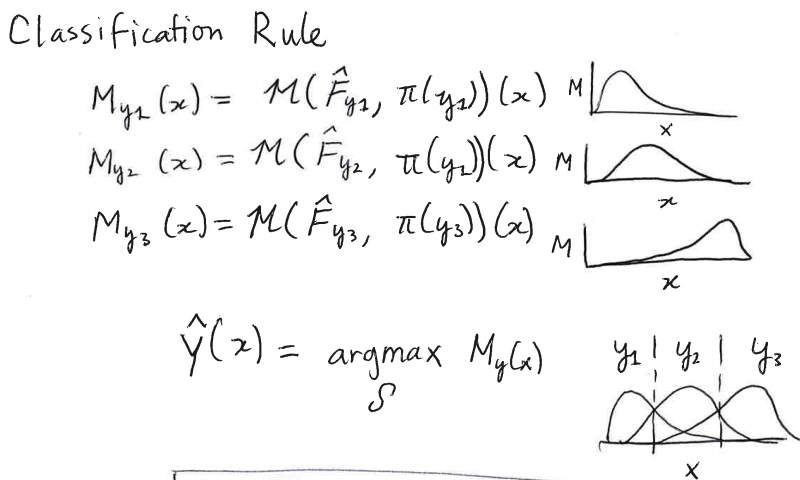
\includegraphics[scale = 0.4]{extrapolation_figures/classification_rule.png}
\caption{Classification rule}\label{fig:classification_rule}
\end{figure}

\begin{figure}[h]
\centering
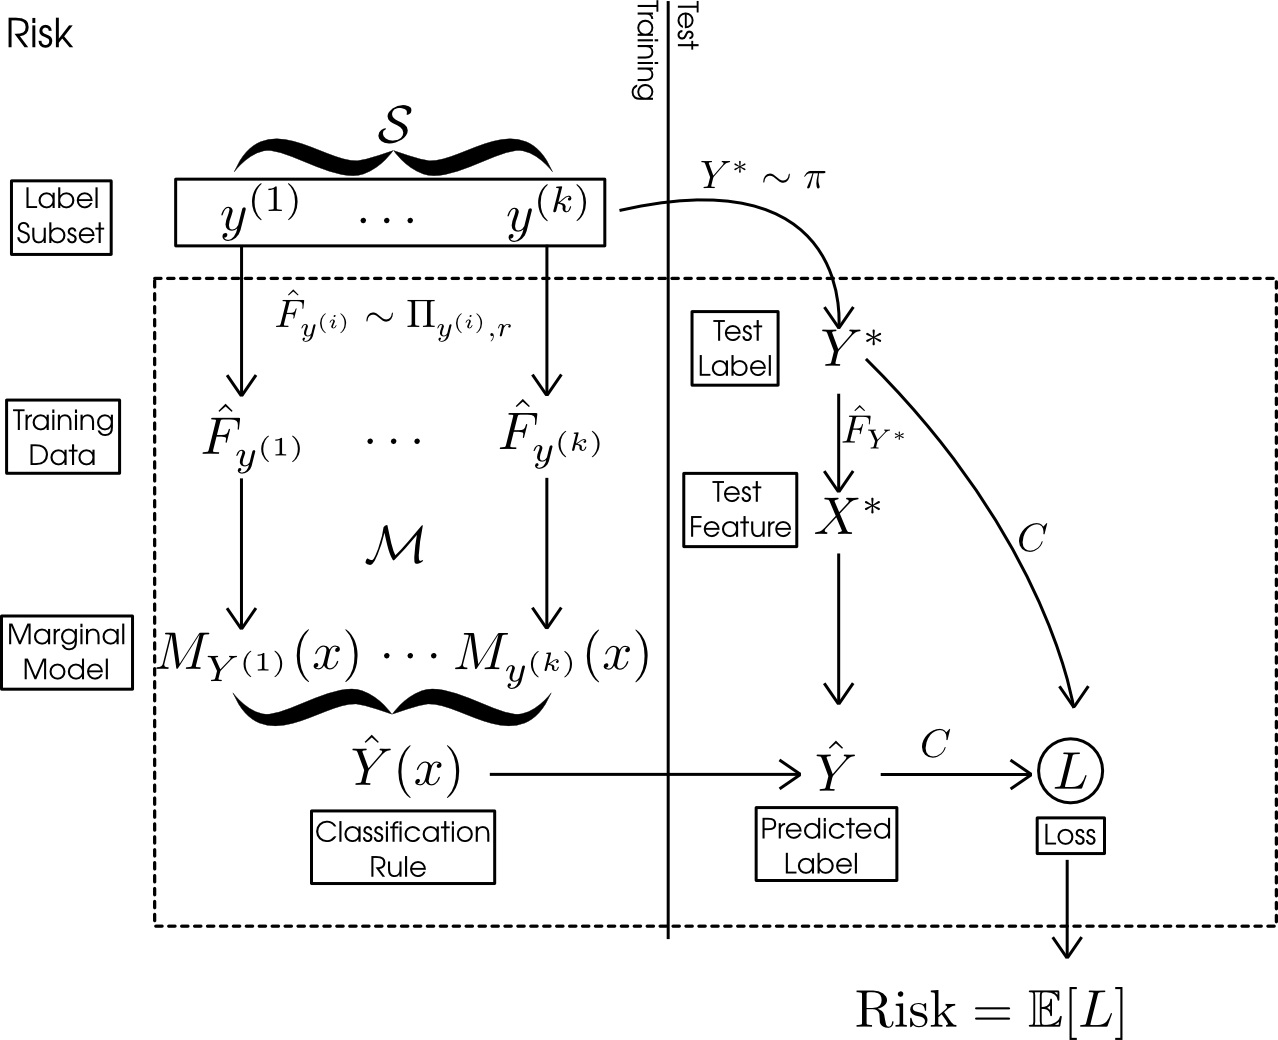
\includegraphics[scale = 0.3]{extrapolation_figures/risk.png}
\caption{Classification risk}\label{fig:risk}
\end{figure}

A \emph{classification task} consists of a subset of labels,
$\mathcal{S} \subset \mathcal{Y}$. Write $\mathcal{S}=\{y_1,\hdots,
y_k\}$, where $k$ is the number of classes.  It is convenient to
decouple the joint distribution of $(X,Y)$ into a prior distribution
over the $k$ labels $\mathcal{S}_k$, and the conditional distribution
of elements, or feature vectors describing them, within a label class
$X|Y=y \sim F_y$.

We would like to identify the sources of randomness in evaluating a
classifier.  First, there is the specific choice of $k$ classes for
the label set. Second, there is randomness in training the classifier
for these classes, which comes from the use of a finite training
set. Third, there is the randomness in the observed accuracy when
testing the classifier on a test set. In order to separate these three
sources, we need to clarify some terms used ambiguously in the
classification literature.

We call a \emph{classification rule} a function $f$ which maps feature
vectors $x \in \mathcal{X}$ to the set of labels $\mathcal{S}$:
\[
f: \mathcal{X} \to \mathcal{S}.
\]
For a random class $Y$ drawn according to the uniform
distribution\footnote{See the discussion for extensions to non-uniform
priors.} on $\mathcal{S}$ and a feature vector drawn under $F_Y$, the
loss of $\ell(f(X),Y)$ is obtained.  The \emph{risk}, or expected
loss, of the classification rule is
\[\text{Risk}(f;\pi,\ell) = \int \ell(f(X),Y)dF_Y d\pi .\]
For now, we will assume a 0--1 loss and a uniform prior over the
labels in $\mathcal{S}$.  Therefore, the risk can be rewritten as
\[\text{Risk}(f;\mathcal{S}, \ell_{01}) = \frac{1}{k}\sum_{y_i\in \mathcal{S}}\Pr(f(X)\neq y_i ; X\sim F_{y_i} ).   \]

The classification rule itself can be seen as a random function that
depends on the sampling of the training set. For convenience, assume
that the training set is composed of $r$ i.i.d examples for
each label $y \in \mathcal{S}$ (a total of $k\times r$).  An
i.i.d. sample of size $r$, $X_1,\hdots, X_r \sim F_y$ can also be
described as an empirical distribution, using the shorthand
$\hat{F}_y$. [[TODO: Should $r$ appear in the notation for $\hat{F}_y$?]].
\[\hat{F}_y = \frac{1}{r}\sum_{i=1}^r \delta_{x_i^{(y)}}.\]

%[[TODO: IS this needed Let $\Pi_{y, r}$ denote the sampling distribution of $\hat{F}_y$. \textcolor{blue}{It is used in the following equation defining Risk(F; pi).}]]

A \emph{classifier} $\mathcal{F}$ is the algorithm or procedure for
producing classification rules given a vector of empirical
distributions $(\hat{F}_y)_{y\in \mathcal{S}}$.  The classifier maps
the empirical distributions to a classification rule $f$
(Figure \ref{fig:classification_rule}).

We can therefore describe the $r$-repeat risk of the model $\mathcal{F}$
as the expected risk of a classification rule $\hat{f}$ trained 
using a sample of size $r$ from each of labels in $\mathcal{S}_k$.
%\mathcal{F}(\hat{F}_{y_1},\hdots, \hat{F}_{y_k})$ trained for the
%classification task on \mathcal{S_k}, $\hat{F}_y \sim \Pi_{y, r}$. 
% NOTE that we suppresed the \ell within Risk_r below
That is,
\[
\text{Risk}_r(\mathcal{F}; \pi) =
\int \text{Risk}(\mathcal{F}(\{\hat{F}_y\}_{y \in \mathcal{S}}; \mathcal{S}, \ell) \prod_{y \in \mathcal{S}} d\Pi_{y, r}(\hat{F}_y).
\]
Figure \ref{fig:risk} illustrates the variables involved in defining
the risk.

The problem of \emph{performance extrapolation} can now be formally
defined as follows: Given a known classification task
$\skone=\{y_1,...,y_{k_1}\}$ with an observed $r$-repeat training set
and $r_{test}$ test set per class, can we estimate the expected
$r$-repeat risk of the classifier $\mathcal{F}$ on a second
classification task with $k_2$ labels?

\subsection{Assumptions}

Implicit in our definition of performance extrapolation is that the
new set of $k_2$ is partially or fully unknown at the time of the
extrapolation. Therefore, the extrapolation must account also for the
randomness in the choice of labels. We will assume that the labels in
the two classification tasks are comparable.

\begin{itemize}
\item[Assumption 1] Let $\skone, \sktwo$ be the label sets
for the first and second classification tasks. Then $\skone, 
\sktwo$ are i.i.d. samples from an infinite population $\pi$.
%\item[Assumption 1B] For $y,y'\sim \pi_Y$, 
%\[P(y=y')=0\]
\end{itemize}

%[[TODO: Assumption 1B is implied by the previous text. Is it really
%necessary as an assumption, or can we deal with it without loss of
%generality. \textcolor{blue}{Assumption 1B is implied by the
%tie-breaking condition, so we can drop it here.}]]

\textbf{Comments:}
\begin{enumerate}
\item These assumption are most easily satisfied by taking $\mathcal{Y}$ 
to be a continuous space and letting $\pi$ be a density over $\mathcal{Y}$. However, a discrete space with a small enough 
probability for the classes would work well. 
\item Note that here we assumed that the label subsets $\skone$ and
$\sktwo$ are independent and disjoint. An alternative
assumption would be that $\skone \subset
\sktwo$ with $\skone$ being a subsample of
$\sktwo$: this assumption can also be addressed, as we will
discuss later.
\item 
In practice, $\skone$ is often a convenience sample meant to be
similar to $\sktwo$. The theory will be relevant insofar as the
assumptions approximate well the true sampling similarity between the
$\skone$ and $\sktwo$.
\item We can imagine other sampling mechanisms designed to make $\skone$ a representative sample from the population, e.g. by stratifying. In this paper we do not discuss these more complex sampling schemes. 
\end{enumerate}

%[TODO: Is the following paragraph really needed? \textcolor{blue}{Somehow we need prior probabilities to be assigned in a sensible way.  An easier alternative would just be to have uniform prior probabilities by default, but this would work really poorly in practice.}]
%[[END of TODO]]

Our analysis will also rely on a property of the classification
model. We do not want the classifier to rely too strongly on
complicated interactions between the labels in the set. We therefore
propose the following property of marginal separability for
classification models:

\begin{definition}
\begin{enumerate}
\item The classification rule $f$ is called a \emph{marginal rule} if 
\[
f(x) = \text{argmax}_{y \in \mathcal{S}} m_y(x),
\]
where the function $m_y$ maps $\mathcal{X}$ to $\mathbb{R}$. 
\item Define a marginal model $\mathcal{M}$ as a mapping from empirical distributions
to margin functions,
\[
\mathcal{M}(\hat{F}_y) = m_y(x).
\]
\item A classifier that produces marginal classification rules
\[
f(x) = \text{argmax}_{y \in \mathcal{S}} m_y(x),
\]
by use of a marginal model, i.e. such that
$m_y=\mathcal{M}(\hat{F}_y)$ for some marginal model $\mathcal{M}$,
is called a \emph{marginal classifier}.
%\item A classifier that produces marginal classification rules
% is called a \emph{marginal model}. 
\end{enumerate}
\end{definition}
In words, a marginal classification rule produces a \emph{margin}, or
score, for each label, and chooses the label with the highest
margin. The marginal model converts empirical distributions
$\hat{F_y}$ over $\mathcal{X}$ into the margin function
$m_y$.  The \emph{marginal} property allows us to prove strong results
about the accuracy of the classifier under i.i.d. sampling assumptions.

%[TODO: Do we need both the marginal model and the marginal classifier? $\mathcal{M}$. \textcolor{blue}{We can omit the definition of marginal classifier here, but later we have to have some discussion of marginal vs non-marginal classifiers.  So we can move the definition to the discussion, maybe.}]]

\textbf{Comments:}
\begin{enumerate}
\item The marginal model includes several popular classifiers.
A primary example for a marginal model is the estimated Bayes
classifier. Let $\hat{f_y}$ be a density estimate obtained from the
empirical distribution $\hat{F_y}$. Then, we can use the estimated
densities of each class to produce the margin functions:
\[ m^{EB}_y(x) = \log(\hat{f_{y}}(x)).\]
%if class probabilities are uniform, or 
%\[m^{EB}_y(x) = \log(\hat{\pi}(y)) + \log(\hat{f_y}(x))\]
%where $\hat{\pi}$ is an estimate of the 
The resulting empirical approximation for the Bayes classifier
(further assuming a uniform prior $\pi$) would be
\[ f^{EB}(x) = \text{argmax}_{y \in \mathcal{S}}(m^{EB}_y(x)).\]
\item Both the Quadratic Discriminant Analysis and the naive Bayes classifiers can be seen as specific instances of an estimated Bayes classifier
\footnote{QDA is the special case of the estimated Bayes classifier when $\hat{f_y}$ is obtained as
the multivariate Gaussian density with mean and covariance parameters estimated from the data.
Naive Bayes is the estimated Bayes classifier when $\hat{f_y}$ is obtained as the product of estimated componentwise marginal distributions
of $p(x_i|y)$}. 
For QDA, the margin function is
given by
\[
m_y^{QDA}(x) = -(x - \mu(\hat{F}_y))^T \Sigma(\hat{F}_y)^{-1} (x-\mu(\hat{F}_y)) - \log\det(\Sigma(\hat{F}_y)),
\]
where $\mu(F) = \int y dF(y)$ and $\Sigma(F) = \int (y-\mu(F))(y-\mu(F))^T dF(y)$.
In Naive Bayes, the margin function is
\[
m^{NB}_y(x) = \sum_{i=1}^n \log \hat{f}_{y, i}(x),
\]
where $\hat{f}_{y, i}$ is a density estimate for the $i$-th component of
$\hat{F}_y$.
\item There are also many classifiers which do not satisfy the marginal property, such as multinomial logistic regression,
multilayer neural networks, decision trees, and k-nearest neighbors.
%[TODO: Examples of classifiers that are not \textcolor{blue}{Such as multinomial logistic regression.}]
%\item[] [TODO: where do you want to treat the empirical vs. true class probabilities? \textcolor{blue}{I guess you are referring to the distinction between population probabilities and sampling probabilities.  If you really want to simplify things, we should just assume that population probabilities, sampling probabilities, and prior probabilities are all uniform, and we can discuss extensions in the same section as for general cost function.}]
\end{enumerate}

\subsection{Definition of average risk}\label{sec:average_risk}

\begin{figure}[h]
\centering
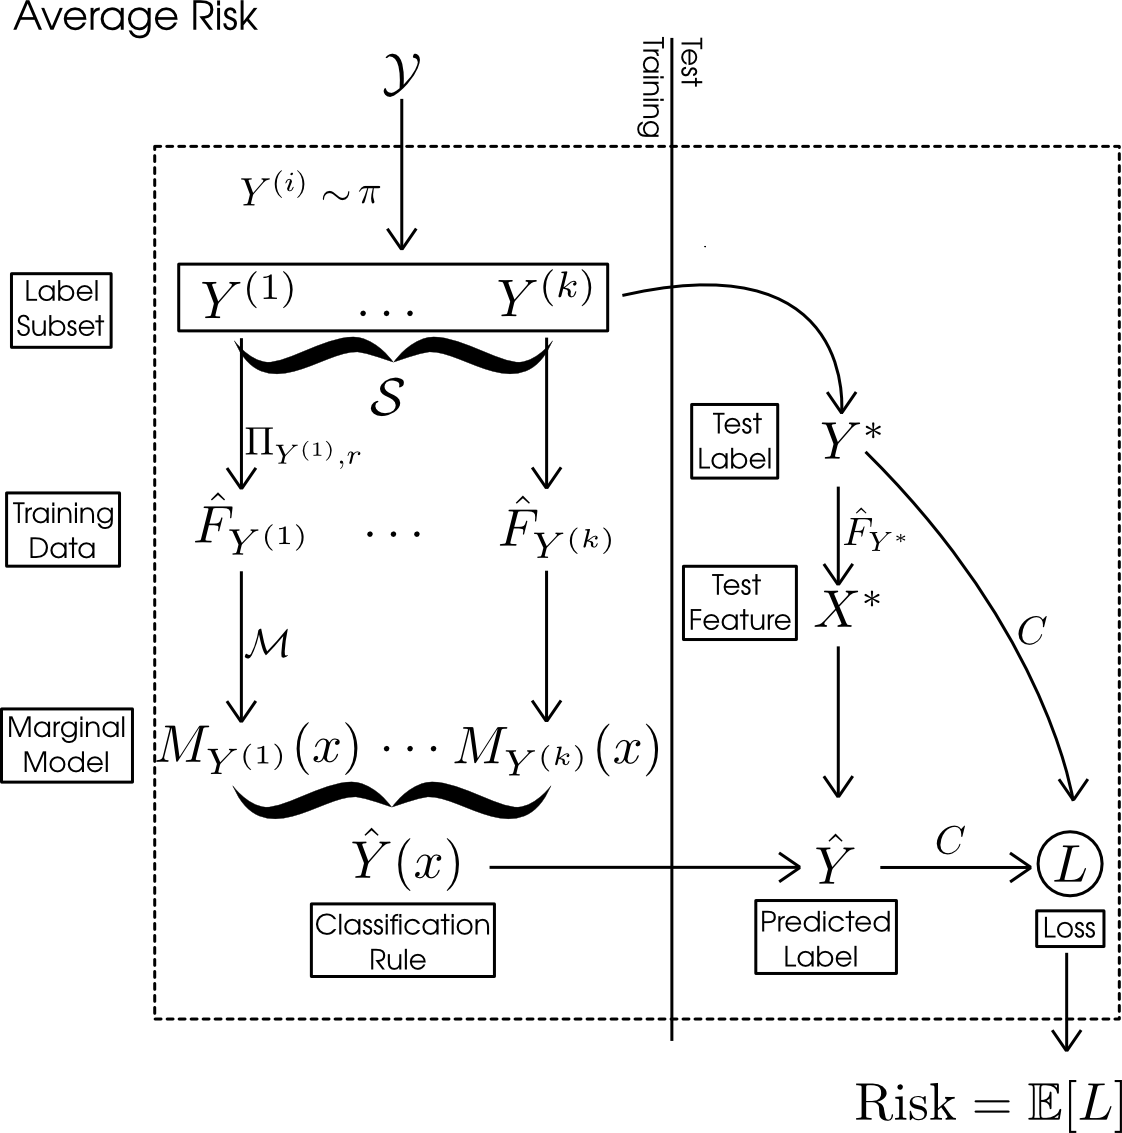
\includegraphics[scale = 0.3]{extrapolation_figures/average_risk.png}
\caption{Average risk}\label{fig:average_risk}
\end{figure}

Since the classification tasks are randomly generated, the $r$-repeat
risk becomes a \emph{random variable} which depends on the random
label subset $\mathcal{S}$.

Therefore, define the $k$-class, $r$-repeat \emph{average risk} of
classifier $\mathcal{F}$ as
\[
\text{AvRisk}_{k, r}(\mathcal{F}) = \E[\text{Risk}_k(\mathcal{F})]
\]
where the expectation is taken over the distribution of $\mathcal{S} =
(Y^{(1)},\hdots, Y^{(k)})$ when $Y^{(i)} \stackrel{iid}{\sim} \text{Unif}(\mathcal{S}).$

As we can see from Figure \ref{fig:average_risk}, the average risk is obtained by averaging
over four randomizations:
\begin{enumerate}
\item[A1.] Drawing the label subset $\mathcal{S}$.
\item[A2.] Drawing the training dataset.
\item[A3.] Drawing $Y^*$ uniformly at random from $\mathcal{S}$.
\item[A4.] Drawing $X^*$ from $F_{X^*}$.
\end{enumerate}

For the sake of developing a better intuition of the average risk, it
is helpful to define a random variable called the \emph{loss}, which
is the cost incurred by a single test instance.  The loss is
determined by quantities from all four randomization steps: the label
subset $\mathcal{S} = \{Y^{(1)},\hdots, Y^{(k)}\}$, the training samples
$\hat{F}_{Y^{(1)}},\hdots, \hat{F}_{Y^{(k)}}$, and the test point $(X^*, Y^*)$.
Formally, we write
\[
L = C(\mathcal{F}(\{\hat{F}_y\}_{y \in \mathcal{S}})(X^*), Y^*).
\]
Now note that the $k$-class, $r$-repeat average risk is the expected loss,
\begin{equation}\label{eq:avrisk_EL}
\text{AvRisk}_{k, r, \nu}(\mathcal{F}) = \E[L] = \E[C(\mathcal{F}(\{\hat{F}_y\}_{y \in \mathcal{S}})(X^*), Y^*)].
\end{equation}
where the expectation is taken over the joint distribution of all the
quantities $\{Y^{(1)},\hdots,
Y^{(k)}, \hat{F}_{Y^{(1)}},\hdots, \hat{F}_{Y^{(k)}}, (X^*, Y^*)\}$.

We will aim to develop a method for estimating the \emph{average
risk}.  In the case where the classification tasks are independently
generated, the average risk is the best predictor (in mean-squared
error) for the (random) risk.


%\subsection{Local polynomial regression}

%Explain background.

%Introduce the notation $\{(w_i, x_i, y_i)\}_{i=1}^n$: ordered triples
%of weight, predictor and response.

\section{Performance extrapolation for marginal classifiers}

Having outlined our assumption for randomized label subsets, the focus
of our theory moves towards understanding the $k$-class average risk:
that is, the expected risk of $\mathcal{F}$ when a random subset
$\mathcal{S}$ of size $k$ is drawn.

We obtain a method for estimating the risk in the second
classification task using data from the first.  The insight behind our
estimation method is obtained via an analysis of the average risk of
the classification task.

\subsection{Toy example}

Let us first illustrate using a toy example the computation of the
average risk, and preview the theory for extrapolating the average
risk.

Let $(Y, X)$ have a bivariate normal joint distribution,
\[
(Y, X) \sim N\left(\begin{pmatrix}0 \\0\end{pmatrix}, \begin{pmatrix}1 & \rho \\ \rho & 1\end{pmatrix}\right),
\]
as illustrated in figure \ref{fig:toy1}(a).
Therefore, for a given randomly drawn label $Y$, the conditional
distribution of $X$ for that label is univariate normal with mean $\rho Y$ and variance $1-\rho^2$:
\[
X|Y = y \sim N(\rho Y, 1-\rho^2).
\]
Supposing we draw $k = 3$ labels $y_1,y_2, y_3$, the classification
problem will be to assign a test instance $X^*$ to the correct label.
The test instance would be drawn from the three-class mixture,
\[
X^* \sim \frac{1}{k}\sum_{i=1}^k p(x|y_i),
\]
as illustrated in figure \ref{fig:toy1}(b, top).  In this toy example, we
ignore the issue of training a classifier from sampled data, and
instead assume that we have access to the \emph{Bayes classification
rule}, or optimal classification rule.  The Bayes rule assigns $X^*$
to the class with the highest density $p(x|y_i)$, as illustrated by
figure \ref{fig:toy1}(b, bottom).

\begin{figure}[h]
\centering
\begin{tabular}{cc}
\multirow{3}{*}{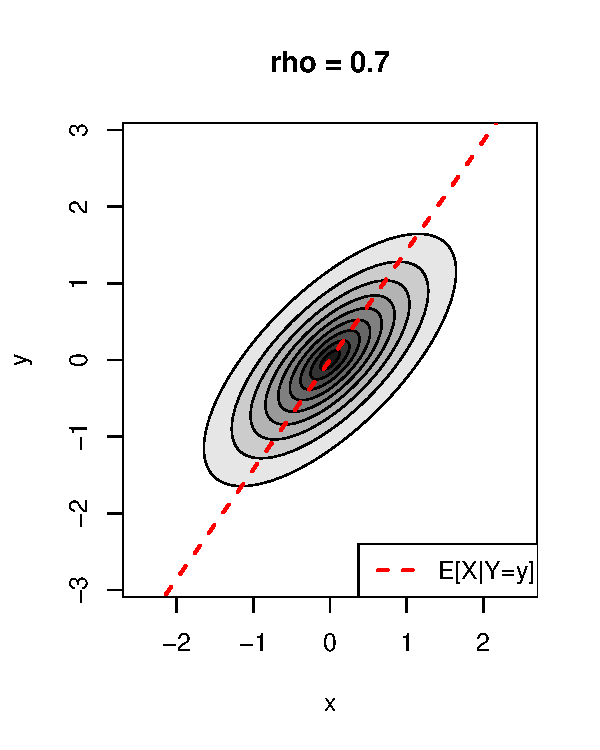
\includegraphics[scale = 0.5, clip = true, trim = 0 0 0 0.5in]{../extrapolation/illus_rho_0_7.pdf}} & \\
& 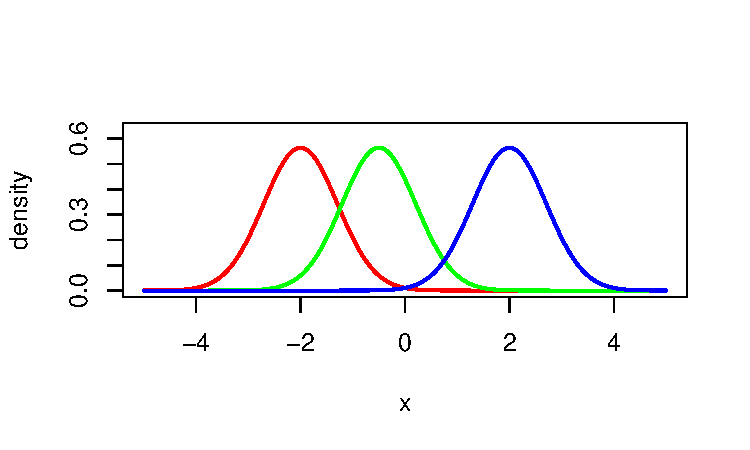
\includegraphics[scale = 0.5, clip = true, trim = 0 0.8in 0 0.8in]{../extrapolation/illus_example1a.pdf}\\
 &  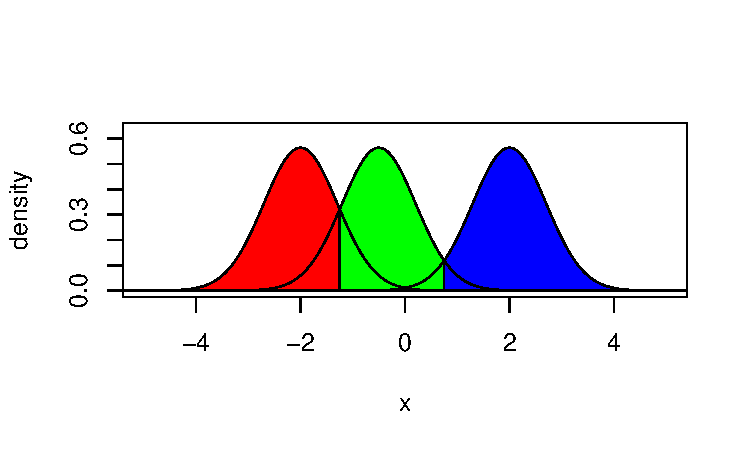
\includegraphics[scale = 0.5, clip = true, trim = 0 0 0 0.5in]{../extrapolation/illus_example1b.pdf}\\
(a) & (b)
\end{tabular}

\caption{
(a) The joint distribution of $(X, Y)$ is bivariate normal with correlation $\rho = 0.7$.
(b) A typical classification problem instance from the bivariate normal model with $k = 3$ classes.
Top: the conditional density of $X$ given label $Y$, for $Y = \{y_1, y_2, y_3\}$.
Bottom: the Bayes classification regions for the three classes.}\label{fig:toy1}
\end{figure}

The risk of the Bayes rule for any label set $\{y_1,\hdots, y_k\}$ is given by
\[
\text{Risk}(y_1,\hdots, y_k) = \frac{1}{k}\sum_{i=1}^k \Pr_{X \sim p(x|y_i)}[p(X|y_i) = \max_{j=1}^k p(X|y_j)].
\]
We numerically computed $\text{Risk}(y_1,\hdots, y_k)$ for randomly
drawn labels $Y_1,\hdots, Y_k \stackrel{iid}{\sim} N(0, 1)$; the
distributions of $\text{Risk}(Y_1,\hdots, Y_k)$ for $k = 2,\hdots, 10$
are illustrated in figure \ref{fig:toy2}.  The $k$-class average risk,
$\text{AvRisk}_k$, in this case, is given by
\[
\text{AvRisk}_k = \E[\text{Risk}(Y_1,\hdots, Y_k)]
\]
for $Y_1,\hdots, Y_k \stackrel{iid}{\sim} N(0, 1)$. The theory
presented in the rest of the section deals with how to analyze the
average risk $\text{AvRisk}_k$ as a function of $k$.  We now proceed
to preview some selected aspects of the theory for the toy example.

\begin{figure}[h]
\centering
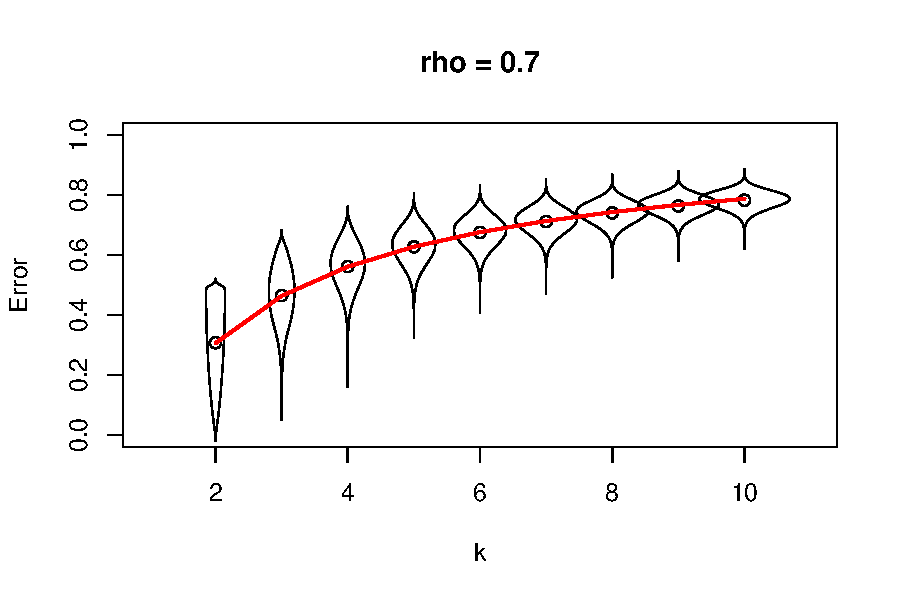
\includegraphics[scale = 0.7, clip = true, trim = 0 0 0 0.5in]{../extrapolation/illus_err_0_7.pdf}

\caption{The distribution of the classification risk for $k = 2,3,\hdots, 10$ for the bivariate normal model with $\rho = 0.7$.
Circles indicate the average classificatin risk; the red curve is the theoretically computed average risk.}\label{fig:toy2}
\end{figure}

For a given test instance $X^*$ drawn from the label $Y^*$, the closer
that $X^*$ is to the center of the correct class distribution, $\rho
Y^*$, the more likely it is to be classified correctly.  Based on this
concept, we define the \emph{conditional accuracy} function $U_x(y)$,
which gives the conditional probability that a test instance $(Y_1,
X_1)$ will be classified correctly in the two-class classification
problem.  One can therefore think of $U_x(y)$ as measuring the
``strength'' of the pair $(y, x)$, with stronger pairs being more
likely to be classified correctly.  Since in the two-class problem,
there is one incorrect class label $Y_2$, the conditional accuracy in
this case is simply the probability that $\rho Y_2$ is closer to $X_1$
than $\rho Y_1$.  Therefore, in this toy example, we can give an
explicit formula
\begin{align*}
U_x(y) &= \Pr[p(x|y) < p(x|Y)]
\\&= \Pr[|\rho Y - x|< |\rho y - x|] 
\\&= \Phi\left(\frac{x + |\rho y - x|}{\rho}\right) - \Phi\left(\frac{x - |\rho y - x|}{\rho}\right),
\end{align*}
where $\Phi$ is the standard normal cumulative distribution function.
Figure \ref{fig:toy3}(a) illustrates the level sets of the function
$U_x(y)$.  The highest values of $U_x(y)$ are near the line $x = \rho
y$ corresponding the to conditional mean of $X|Y$: as one moves
farther from the line, $U_x(y)$ decays.  Note however that large
values of $(y, x)$ (with the same sign) result in larger values of
$U_x(y)$ since it becomes unlikely for $Y_2 \sim N(0,1)$ to exceed
$Y_1 = y$.

Now define the random variable $U = U_X(Y)$ for $(X, Y)$ drawn from
the joint distribution.  An important object in our theory is the
cumulative distribution function
\footnote{Note however that $\bar{D}(u)$ is only defined as the cumulative
distribution function of $U$ in the class of zero-one loss--the
definition for general cost functions is somewhat more involved, as we
will see.}
of $U$, written as
\[
\bar{D}(u) = \Pr[U \leq u].
\]
The function $\bar{D}$ is illustrated in
figure \ref{fig:toy3}(b) for the current example with $\rho = 0.7$.
The red curve in figure \ref{fig:toy2} was computed using the formula
\[
\text{AvRisk}_k = (k-1) \int \bar{D}(u) u^{k-2} du.
\]

\begin{figure}[h]
\centering
\begin{tabular}{cc}
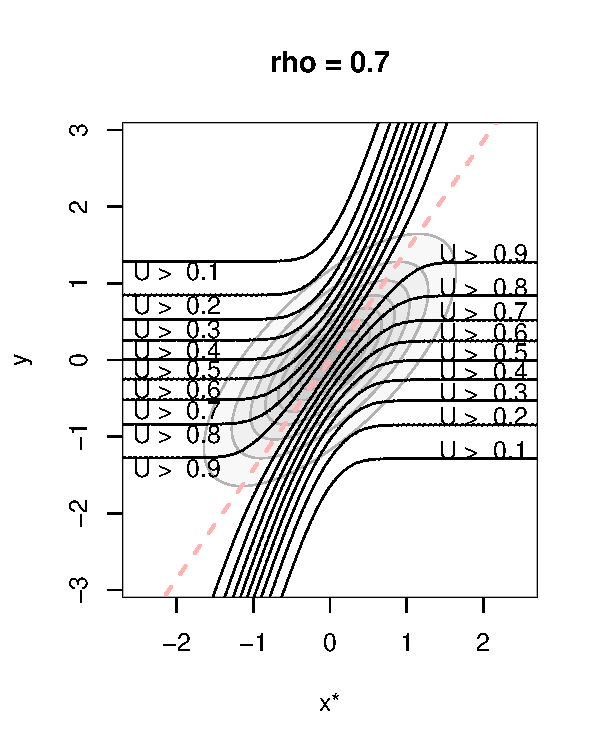
\includegraphics[scale = 0.6, clip = true, trim = 0.1in 0 0 0.8in]{../extrapolation/illus_ufunc_0_7.pdf} &
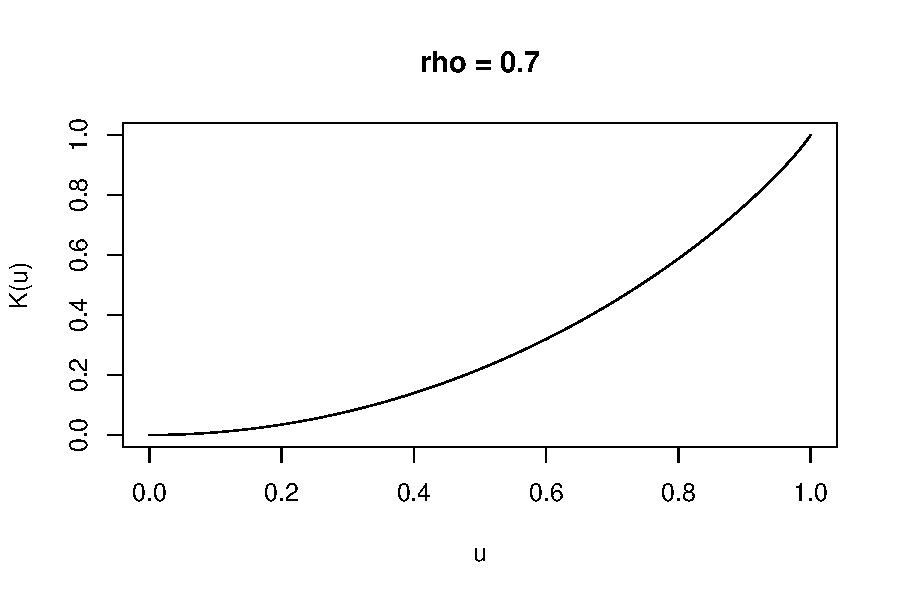
\includegraphics[scale = 0.65, clip = true, trim = 0 -0.3in 0 0.5in]{../extrapolation/illus_kfunc_0_7.pdf}\\
(a) & (b)
\end{tabular}

\caption{
(a) The level curves of the function $U_x(y)$ in the bivariate normal model with $\rho = 0.7$.
(b) The function $\bar{D}(u)$, which gives the cumulative distribution function of the random variable $U_Y(X)$.}\label{fig:toy3}
\end{figure}

It is illuminating to consider how the average risk curves and the
$\bar{D}(u)$ functions vary as we change the parameter $\rho$.  Higher
correlations $\rho$ lead to lower classification risk, as seen in
figure \ref{fig:toy4}(a), where the risk curves are shifted downward as
$\rho$ increases from 0.3 to 0.9.  The conditional accuracy $U_y(x)$
tends to be higher on average as well, which leads to lower values of
the cumulative distribution function--as we see in
figure \ref{fig:toy4}(b), where the function $\bar{D}(u)$ becomes smaller
as $\rho$ increases.

In section \ref{sec:estimation}, when we consider approximating
$\bar{D}(u)$ by polynomials, or some other function basis, it becomes
relevant to consider how well $\bar{D}(u)$ can be approximated by such
bases in realistic problems.  We see in figure \ref{fig:toy4}(c) that,
at least in this toy problem, $\bar{D}(u)$ is well-aproximated by
low-order polynomials.  However, the approximation becomes less
adequate as $\rho$ increases.  We can see visually why this is the
case: as $\rho$ increases, the curvature of $\bar{D}(u)$ near $u = 1$
increases.  Hence, higher-degree polynomials become needed to capture
the behavior near $u = 1$.  More generally, we observe that in cases
where classes are relatively well-separated, it becomes necessary to
use increasingly precise approximations in order to extrapolate the
average risk.

\begin{figure}[h]
\centering
\begin{tabular}{ccc}
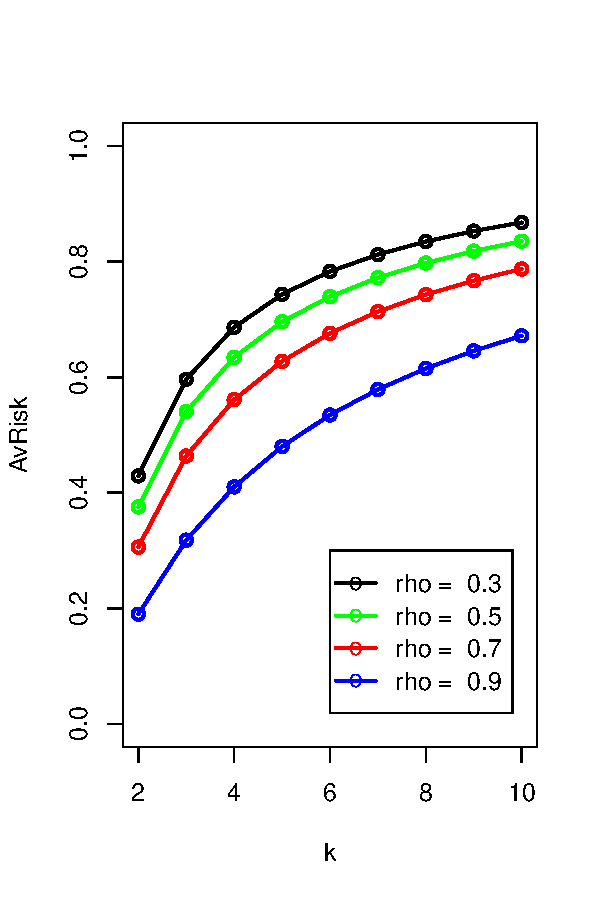
\includegraphics[scale = 0.45, clip = true, trim = 0.05in 0 0.2in 0.6in]{../extrapolation/illus_rhos_avrisk.pdf} &
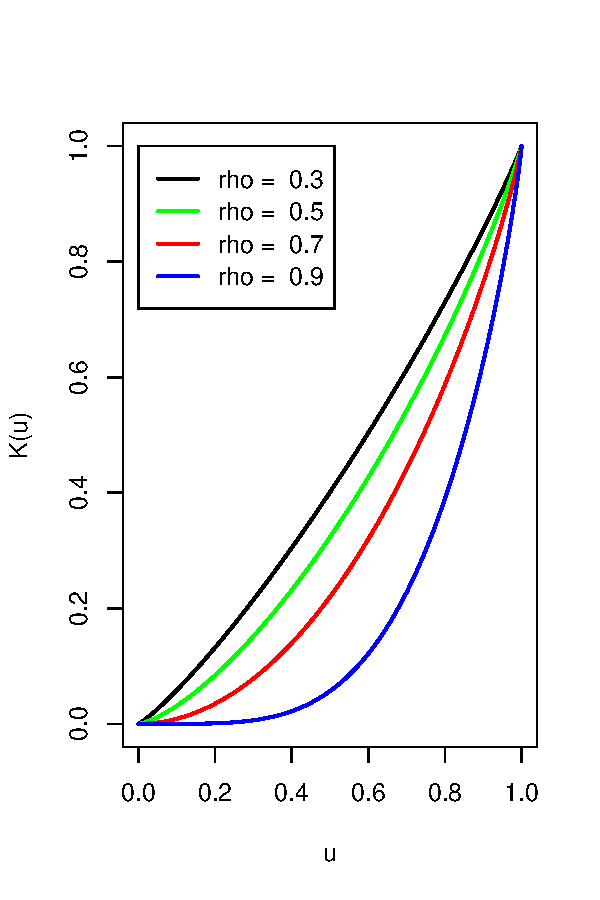
\includegraphics[scale = 0.45, clip = true, trim = 0.05in 0 0.2in 0.6in]{../extrapolation/illus_rhos_Kfunc.pdf} &
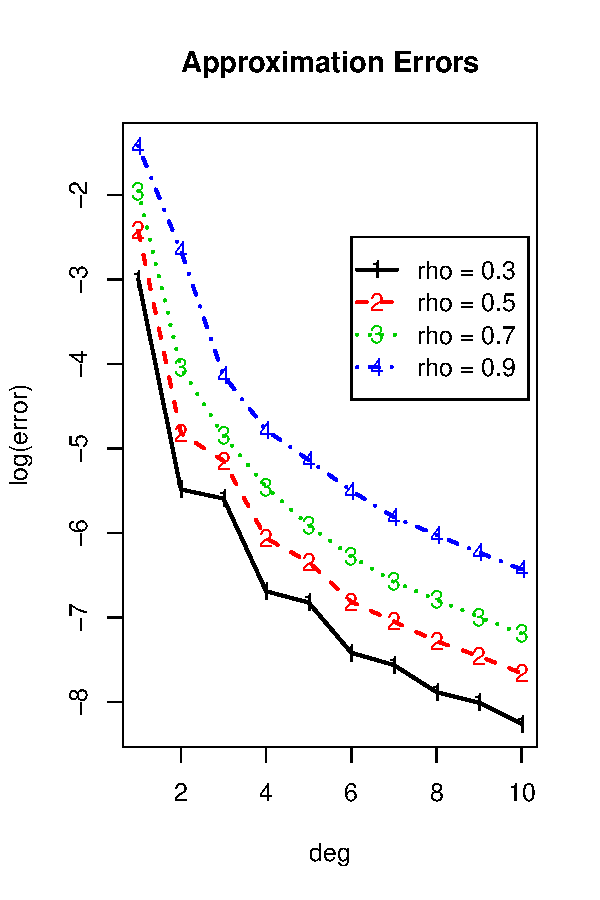
\includegraphics[scale = 0.45, clip = true, trim = 0.05in 0 0.2in 0.6in]{../extrapolation/illus_approx_errors.pdf}\\
(a) & (b) & (c)
\end{tabular}

\caption{
The (a) average risk, (b) $\bar{D}(u)$ function for $k = 2,\hdots, 7$ for the bivariate normal model with $\rho \in \{0.3, 0.5, 0.7, 0.9\}$.
(c) The $d$-degree $\ell_\infty$ polynomial approximation error for $\bar{D}(u)$ for the bivariate normal model with $\rho \in \{0.3, 0.5, 0.7, 0.9\}$.
}\label{fig:toy4}
\end{figure}

\subsection{Easy special cases}

Let us first mention two easy special cases, which can be handled
using existing machine learning methodology.

\subsubsection{Equal numbers of classes}

In the special case where $k_1 = k_2 = k$: that is, where the label
subsets $\mathcal{S}_1$ and $\mathcal{S}_2$ are the same size, it is
clear to see that any unbiased estimate of the risk of the classifier
$\mathcal{F}$ for the first classification problem is an unbiased
estimate of the average $k$-class risk.  The \emph{test risk}
gives one such unbiased estimate of the average $k$-class risk.

Recall that the data consists of class labels $y^{(i)}$ for $i =
1,\hdots, k_1$, as well as training sample $\hat{F}_{y^{(i)}}$ and
test sample $(x_1^{(i)},\hdots, x_{r_{test}}^{(i)})$ for $i =
1,\hdots, k_1$.

For any given test observation $x_j^{(i)}$, we obtain the predicted
label $\hat{y}_j^{(i)}$ by computing the margin for each class,
\[
M_{i,j,\ell} = \mathcal{M}(\hat{F}_{y^{(\ell)}})(x_j^{(i)}) =  m_{y^{(\ell)}}(x_i^{(j)}),
\]
for $\ell = 1,\hdots, k$,
and by finding the class with the highest margin $M_{i, j, \ell}$,
\[
\hat{y}_j^{(i)} = y_{\argmax_\ell M_{i, j, \ell}}.
\]
The test risk is the average cost over test observations,
\begin{equation}
\text{Test Risk} = \frac{1}{r_{test}k} \sum_{i=1}^k \sum_{j=1}^{r_{test}} C(\hat{y}_j^{(i)}, y^{(i)}).
\end{equation}
For each test observation, define the ranks of the margins by
\[
R_{i,j,\ell} = \sum_{m \neq \ell} I\{M_{i,j,\ell} \geq M_{i, j, m}\}.
\]
Therefore, $\hat{y}_j^{(i)}$ is equal to $\ell$ if and only if $R_{i,j,\ell} = k$.
Thus, an equivalent expression for test risk is
\begin{equation}\label{eq:test_risk}
\text{Test Risk} = \frac{1}{r_{test}k} \sum_{i=1}^k \sum_{\ell=1}^k \sum_{j=1}^{r_{test}} C_{ij} I\{R_{ij\ell} = k\}.
\end{equation}
where
\[
C_{ij} = C(y^{(j)}, y^{(i)}).
\]

Besides the test risk, other methods, such as cross-validation, can
also be used to obtain estimates of the average $k$-class risk.

\subsubsection{Fewer classes}

Suppose we have data for $k_1$ classes, and we wish to estimate
$\text{AvRisk}_{k_2}$ for $k_2 \leq k_1$.  Let $\mathcal{S}_1
= \{y_1,\hdots,y_{k_1}\}$.  To obtain a classification problem with
$k_2$ classes, we can simply pick a subset $S$ of size $k_2$ from
$\mathcal{S}_1$, and throw away all the training and test data from the
other classes $\mathcal{S}\setminus S$.  Then, the test
risk \eqref{eq:test_risk} gives an unbiased estimate of the
$\text{AvRisk}_{k_2}$.

Of course, one could obtain a better estimator of the average risk by
averaging over all the subsets $S \subset \mathcal{S}_1$ of size
$k_2$.  For general classifiers, this may require retraining a
classifier over each subset.  However, for marginal classifiers, one
can compute the average test risk over all ${k_1}\choose{k_2}$ subsets
easily.

The reason why the efficient computation is possible is because the
test risk for each subproblem can be determined by looking at the
margins $M_{i, j, \ell}$, which remain the same as long as both $i$
and $\ell$ are included in the subsample $S$.

The computational trick is to look at each combination of test
observation $x_j^{(i)}$ and class label $y^{(\ell)}$, and to count the
number of subsets $N_{i, j, \ell}$ where (i) both $i$ and $\ell$ are
included in $S$, and (ii) $\hat{y}_j^{(i)} = y^{(\ell)}$.  Then it
should be clear that the average test risk over all subsets is equal
to
\begin{equation}\label{eq:avtestrisk}
\text{AvTestRisk}_{k_2} = \frac{1}{{{k_1}\choose{k_2}}}\frac{1}{r_{test}k_2} \sum_{i=1}^{k_1} \sum_{\ell\neq i} \sum_{j=1}^{r_{test}} C_{i\ell}N_{i, j, \ell}.
\end{equation}
Now it is just a matter of simple combinatorics to compute
$N_{i,j,\ell}$.  We require both $y^{(i)}$ and $y^{(\ell)}$ to be
included in $S$.  This implies that if $M_{i,j,i} > M_{i,j,\ell}$,
then $y^{(\ell)}$ will never have the highest margin in any of those
subsets, so $N_{i,j,\ell} = 0$.

Otherwise, there are $R_{i,j,\ell} - 1$ elements in $\mathcal{S}_1$
with a lower margin than $y^{(\ell)}$.  Since $i \neq \ell$, then there
are $k_2-2$ elements in $S \setminus \{i, \ell\}$, so therefore $N_{i,
j, \ell} = {{R_{i,j,\ell} - 2}\choose{k_2 - 2}}$.  Therefore, we can write
\begin{equation}\label{eq:avtestrisk_nil}
N_{i,j,\ell} = I\{R_{i,j,\ell} > R_{i,j,i}\}{{R_{i,j,\ell} -2}\choose{k_2 - 2}}
\end{equation}

Therefore, the challenging case is when $k_2 > k_1$: we want to
predict the performance of the classification model in a setting with
more labels than we currently see in the training set.

\subsection{Analysis of the average risk}

As we pointed out in the previous section, the challenging case for
the analysis is the ``undersampled'' regime where we wish to predict
the loss on a larger label set.  Given data with $k_1$ classes, we
already have means to estimate the average risk for all $k \leq k_1$,
so the challenge is to understand how the risk will ``extrapolate'' to
$k > k_1$.  Hence, the goal of the current analysis is to isolate the
effect of $k$, the size of the label subset, on the average risk.

The result of our analysis is to expose the average risk
$\text{AvRisk}_{k, r}$ as the weighted average of a function
$\bar{D}(u)$, where $\bar{D}(u)$ is independent of $k$, and where $k$
only changes the weighting.  The result is stated as follows.

\begin{theorem}\label{theorem:avrisk_identity}
Suppose $\pi$, $\{F_y\}_{y \in \mathcal{Y}}$ and marginal classifier
$\mathcal{F}$ satisfy the tie-breaking condition.  Then, under the
definitions \eqref{eq:U_function}, \eqref{eq:Kfunc},
and \eqref{eq:Kbar}, we have
\begin{equation}\label{eq:avrisk_identity}
\text{AvRisk}_{k, r} = (k-1) \int \bar{D}(u) u^{k-2} du.
\end{equation}
\end{theorem}

The tie-breaking condition referred in the theorem is defined as follows.
\begin{itemize}
%\item 
%\emph{Scaling property of margins}: if $\mathcal{M}(\hat{F}_1, \pi_1)(x) >
%\mathcal{M}(\hat{F}_2, \pi_2)(x)$ then also $\mathcal{M}(\hat{F}_1,
%c\pi_1)(x) > \mathcal{M}(\hat{F}_2, c\pi_2)(x)$.
\item 
\emph{Tie-breaking condition}: for all $x \in \mathcal{X}$,
$\mathcal{M}(\hat{F}_Y)(x) = \mathcal{M}(\hat{F}_{Y'})(x)$
with zero probability for $Y, Y'$ independently drawn from $\pi$.
\end{itemize}
%The scaling property of margins is satisfied by most of the marginal
%classifiers which are used in practice, and as such we do not consider
%it to be a strong assumption.  Meanwhile, 
The tie-breaking condition is a technical assumption which allows us
to neglect the specification of a tie-breaking rule in the case that
margins are tied.  In practice, one can simply break ties randomly,
which is mathematically equivalent to adding a small amount of random
noise $\epsilon$ to the function $\mathcal{M}$.

Our strategy is to analyze the average risk \eqref{eq:avrisk_EL} by
means of \emph{conditioning on} the true label and its training
sample, $(y^*, \hat{F}_{y^*})$, and the test feature $x^*$
while \emph{averaging} over all the other random variables.  Define
the \emph{conditional average risk} $\text{CondRisk}_k((y^*, \hat{F}_{y^*}), x^*)$ as
\[
\text{CondRisk}_k((y^*, \hat{F}_{y^*}), x^*) = \E[L|Y^*=y^*, X^* = x^*, \hat{F}_{Y^*} = \hat{F}_{y^*}].
\]
Figure \ref{fig:conditional_risk} illustrates the variables which are
fixed under conditioning and the variables which are randomized.
Compare to figure \ref{fig:average_risk}.

Without loss of generality, we can write the label subset $\mathcal{S}
= \{Y^*, Y^{(1)},\hdots, Y^{(k-1)}\}$.  Note that due to independence,
$Y^{(1)},\hdots, Y^{(k-1)}$ are still i.i.d. from $\pi$ even
conditioning on $Y^* = y^*.$ Therefore, the conditional risk can be
obtained via the following alternative order of randomizations:
\begin{enumerate}
\item[C0.] 
Fix $y^*, \hat{F}_y^*,$ and $x^*$.  Note that $M_{y^*}(x^*)
= \mathcal{M}(\hat{F}_{y^*})(x^*)$ is also fixed.
\item[C1.]
Draw the \emph{incorrect labels} $Y^{(1)},\hdots, Y^{(k)}$ i.i.d. from
$\pi$.  (Note that $Y^{(i)} \neq y^*$ with probability 1 due to the
continuity assumptions on $\mathcal{Y}$ and $\pi$.)
\item[C2.]
Draw the training samples for the incorrect labels
$\hat{F}_{Y^{(1)}},\hdots, \hat{F}_{Y^{(k-1)}}$.  This determines
\[
\hat{Y} = \argmax_{y \in \mathcal{S}} M_y(x^*)
\]
and hence
\[
L = C(\hat{Y}, y^*).
\]
\end{enumerate}
Compared to four randomization steps listed in
section \ref{sec:average_risk}, we have essentially conditioned on
steps A3 and A4 and randomized over steps A1 and A2.

%Let $G$ denote the joint distribution over $(X, Y)$ obtained by
%drawing $Y \sim \pi_0$ and $X \sim F_Y$.  Since $Y^*$ has the marginal
%distribution $\pi_0$, it follows that
%\begin{equation}\label{eq:rk_eq}
%\text{Average Risk}_k(\mathcal{F}) = \int \int R_k(y^*, x^*) dG(x^*, y^*).
%\end{equation}
%What we have done is to rewrite the average risk as the expectation of
%$R_k$, which depends on $k$, according to a measure $G$ which does
%\emph{not} depend on $k$.%

\begin{figure}[h]
\centering
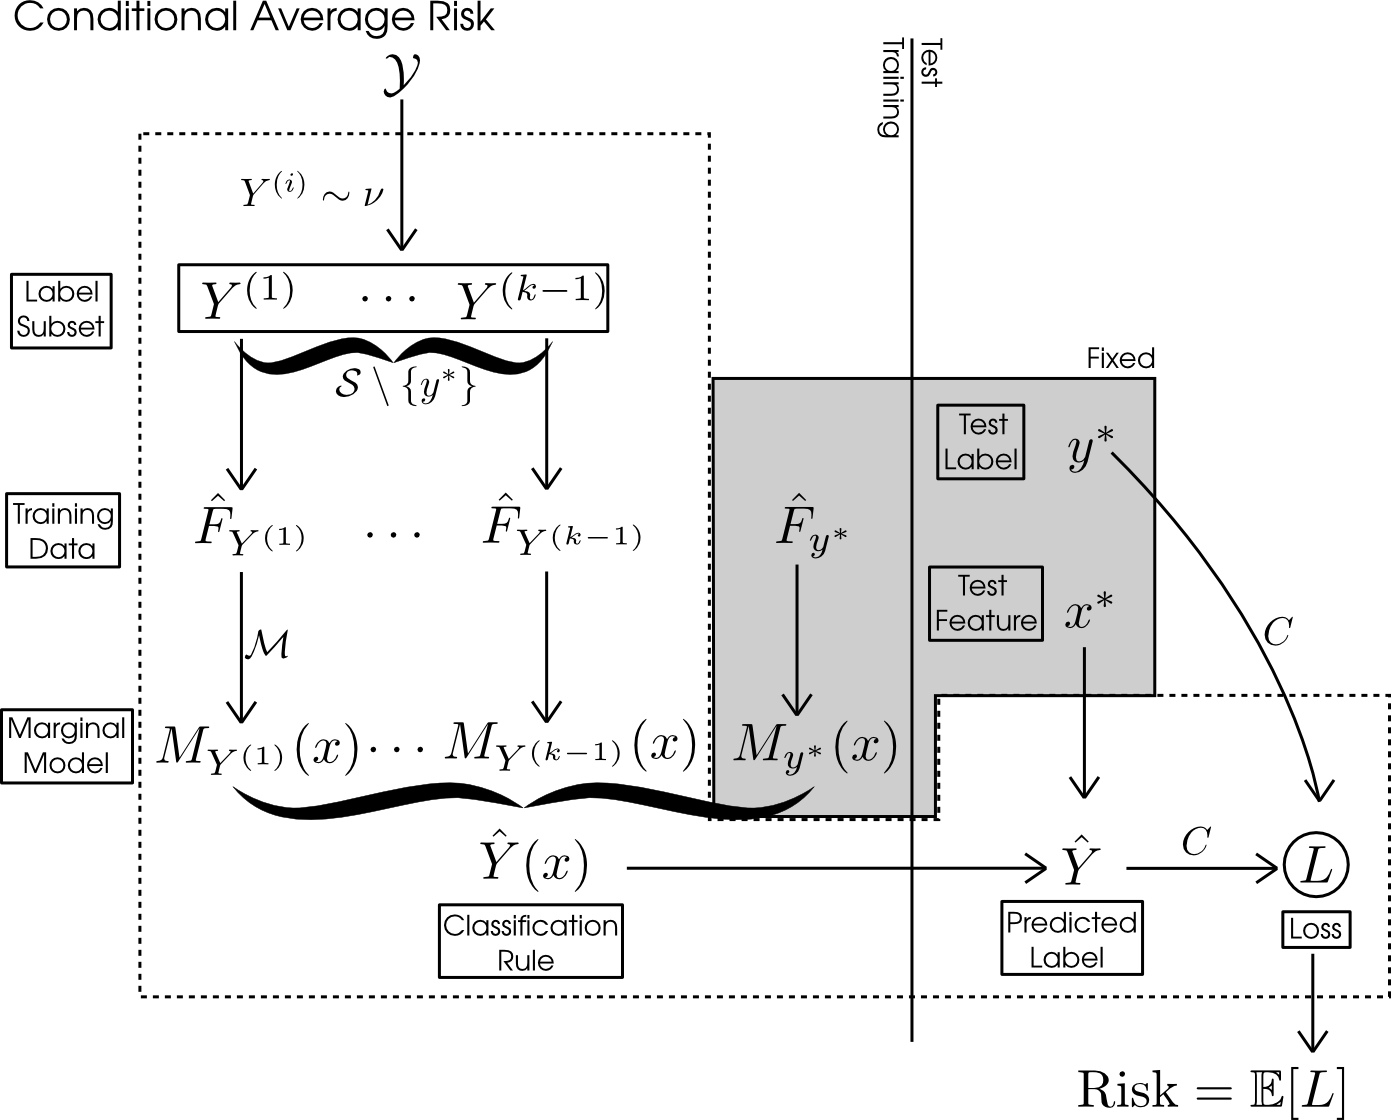
\includegraphics[scale = 0.3]{extrapolation_figures/conditional_risk.png}
\caption{Conditional average risk}\label{fig:conditional_risk}
\end{figure}

%However, we will further decompose $R_k$ into $k$-dependent and $k$-independent components.
%Having defined the conditional average risk, we will now further
%decompose it to expose its dependence on $k$.
Now, in order to analyze the $k$-class behavior of the conditional
average risk, we begin by considering the \emph{two-class} situation.

In the two-class situation, we have a true label $y^*$ and one
incorrect label, $Y$.  Define the \emph{U-function}
$U_{x^*}(y^*, \hat{F}_{y^*})$ as the \emph{probability of correct
classification} in the two-class case.
The classification is correct if the margin
$M_{y^*}(x^*)$ is greater than the margin $M_Y(x^*)$, and incorrect
otherwise.  
Since we are fixing $x^*$ and $(y^*, \hat{F}_{y^*})$, the
probability of correct classification is obtained by taking an expectation:
\begin{align}\label{eq:U_function}
U_{x^*}(y^*, \hat{F}_{y^*}) &= \Pr[M_{y^*}(x^*) > \mathcal{M}(\hat{F}_Y)(x^*)]
\\&= \int_{\mathcal{Y}} 
I\{
M_{y^*}(x^*) > \mathcal{M}(\hat{F}_{y})(x)
\}
d\Pi_{y, r}(\hat{F}_y)
d\pi(y).
\end{align}
See also figure \ref{fig:U_function} for an graphical illustration of
the definition.

\begin{figure}[h]
\centering
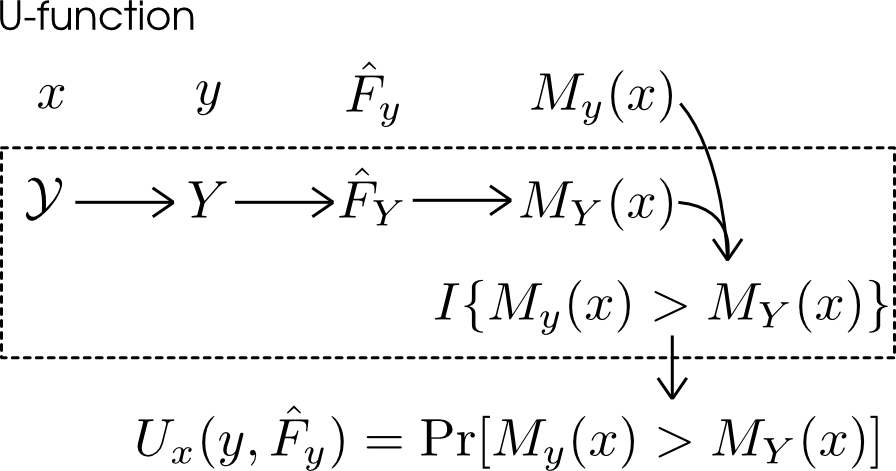
\includegraphics[scale = 0.4]{extrapolation_figures/U_function.png}
\caption{U-functions}\label{fig:U_function}
\end{figure}

An important property of the U-function, and the basis for its name,
is that the random variable $U_x(Y, \hat{F}_Y)$ for $Y \sim \pi$ and
$\hat{F}_Y \sim \Pi_{Y, r}$ is uniformly distributed for all
$x \in \mathcal{X}$.  This is proved in Lemma \ref{lemma:U_function}
in the appendix.

Now, we will see how the U-function allows us to understand the
$k$-class case.  Suppose we have true label $y^*$ and incorrect labels
$Y^{(1)},\hdots, Y^{(k-1)}$.  Note that the U-function
$U_{x^*}(y, \hat{F}_y)$ is monotonic in $M_y(x^*)$.  Therefore,
\[
\hat{Y} = \argmax_{y \in \mathcal{S}} M_y(x^*) = \argmax_{y \in \mathcal{S}} U_{x^*}(y, \hat{F}_y).
\]
Therefore, we have a correct classification if and only if the U-function value for the correct label
is greater than the maximum U-function values for the incorrect labels:
\[
\Pr[\hat{Y} = y^*] = \Pr[U_{x^*}(y^*, \hat{F}_{y^*}) > \max_{i=1}^{k-1} U_{x^*}(Y^{(i)}, \hat{F}_{Y^{(i)}})] =  \Pr[u^* > U_{max}].
\]
where $u^* = U_{x^*}(y^*, \hat{F}_{y^*})$ and $U_{max, k-1}
= \max_{i=1}^{k-1} U_{x^*}(Y^{(i)}, \hat{F}_{Y^{(i)}})$.  But now,
observe that we know the distribution of $U_{max, k-1}$!  Since
$U_{x^*}(Y^{(i)}, \hat{F}_{Y^{(i)}})$ are i.i.d. uniform, we know that
\begin{equation}\label{eq:umax_beta}
U_{max, k-1} \sim \text{Beta}(k-1, 1). 
\end{equation}
We now have the insights needed to analyze the simplest special case: zero-one loss.
\newline

\noindent \emph{Special case: 0-1 loss}.
For zero-one loss, which is $C(y, y') = I\{y = y'\}$, we have $L=1$ if
and only if $U_{max} > u^*$ and $L=0$ otherwise.  Therefore, the
conditional average risk is
\[
\text{CondRisk}_k((y^*, \hat{F}_{y^*}), x^*) = \Pr[U_{max} > u^*] = \int_{u^*}^1 (k-1) u^{k-2} du.
\]
Now the average risk can be obtained by integrating over the distribution of $U^* = U_{x^*}(y^*, \hat{F}_{y^*})$.
We have
\begin{align*}
\text{AvRisk}_k &= \E[ \int_{U^*}^1 (k-1) u^{k-2} du] 
\\&= \E[\int_0^1 I\{u \geq U^*\} (k-1) u^{k-2} du ]
\\&= (k-1) \int_0^1 \Pr[U^* \leq u] u^{k-2} du.
\end{align*}
Or equivalently,
\[
\text{AvRisk}_{k, r, \nu}((y^*, \hat{F}_{y^*}), x^*) = (k-1) \int \bar{D}(u) u^{k-2} du.
\]
where $\bar{D}(u)$ denote the cumulative distribution function of $U^*$ on $[0,1]$:
\[
\bar{D}(u) = \Pr[U_{x^*}(y^*, \hat{F}_{y^*}) \leq u].
\]
We have expressed the average risk expressed as a weighted integral of
a certain function $\bar{D}(u)$ defined on $u \in [0,1]$.  We have
clearly isolated the part of the average risk which is independent of
$k$--the univariate function $\bar{D}(u)$, and the part which is
dependent on $k$--which is the density of $U_{max}$.

In section \ref{sec:estimation}, we will develop estimators of
$\bar{D}(u)$ in order to estimate the $k$-class average risk.
But now let us return to the general case.
\newline

\noindent \emph{General loss functions.}
The case for general cost functions is somewhat more complicated,
since knowledge of $U_{max}$ is not sufficient to determine $L$.  In
short, this is because $U_{max}$ by itself is insufficient to
determine $\hat{Y}$, and therefore $L=C(\hat{Y}, y^*)$.  However, we
can resolve this issue by noting that for the purposes of computing
the expected loss, it suffices to have the \emph{conditional
distribution} of $\hat{Y}$ given $U_{max}$.  Even though $U_{max}$
does not deterministically map onto a unique $\hat{Y}$, it determines
a conditional distribution of $\hat{Y}$ which allows us to compute
$\E[L|U_{max}, x^*, y^*, \hat{F}_{y^*}]$.

Now, a key fact is that the conditional distribution of $\hat{Y}$
given $U_{max}$ \emph{does not depend} on $k$.  To see this fact,
suppose without loss of generality that $\hat{Y} = Y^{(k-1)}.$ Then
the joint density of $Y^{(1)},\hdots, Y^{(k-1)}$ given $U_{max} =
u$ can be written
\[
p(y^{(1)},\hdots, y^{(k-1)}) \propto 
\pi(y^{(k-1)})\frac{d}{dt}\Pr[U_{x^*}(y^{(k-1)}, \hat{F}_{y^{(k-1)}}) \leq t]|_{t=u}
\prod_{i=1}^{k-2}\pi(y^{(i)})\Pr[U_{x^*}(y^{(k-1)}, \hat{F}_{y^{(k-1)}}) < u].
\}
\]
up to a normalizing constant.  Note that the term
$\frac{d}{dt}\Pr[U_{x^*}(y^{(k-1)}, \hat{F}_{y^{(k-1)}}) \leq t]$ is the
density of the random variable
$U_{x^*}(Y^{(k-1)}, \hat{F}_{Y^{(k-1)}})$. From the density, we can see
that $Y^{(1)},\hdots, Y^{(k-1)}$ are conditionally independent given
$U_{max} = u$, hence the marginal density of $\hat{Y}=Y^{(k-1)}$ can
be written
\[
p(\hat{y}) \propto \pi(\hat{y})\frac{d}{dt}\Pr[U_{x^*}(y^{(k-1)}, \hat{F}_{y^{(k-1)}}) \leq t]|_{t=u}.
\]

The only property of the conditional distribution of $\hat{Y}|U_{max} = u$ that is needed is
the expectation of $L = C(\hat{Y}, y^*)$.  Therefore, define the \emph{conditional expected loss} $D((y^*, \hat{F}_{y^*}), x^*, u)$ by
\begin{equation}\label{eq:Kfunc}
D((y^*, \hat{F}_{y^*}), x^*, u) = \begin{cases} 0 \text{ if } u < u^*\\
\E[C(\hat{Y}, y^*)|U_{max} = u, x^*, y^*, \hat{F}_{y^*}] \text{ otherwise.}
\end{cases}
\end{equation}
We have the two cases $u < u^*$ and $u > u^*$ since when $U_{max} <
u^*$, the correct label is chosen and the loss is zero.  Otherwise, an
incorrect label is chosen, and the expected loss must be calculated
using the conditional distribution of $\hat{Y}$.

Again, since the conditional distribution of $\hat{Y}|U_{max}, x^*,
(y^*, \hat{F}_{y^*})$ is independent of $k$, the conditional cost
function is also independent of $k$.

With the conditional cost function and the distribution of $U_{max}$ both in hand, we can compute the average conditional risk
\[
\text{CondRisk}_k((y^*, \hat{F}_{y^*}), x^*) = (k-1) \int D((y^*,\hat{F}_{y^*}), x^*, u) u^{k-2} du.
\]
Now the average risk can be obtained by integrating over $(Y^*, \hat{F}_{Y^*}),$ and $X^*$.
\[
\text{AvRisk}_{k, r} = (k-1) \int \bar{D}(u) u^{k-2} du.
\]
where
\begin{equation}\label{eq:Kbar}
\bar{D}(u) = \int D((y^*,\hat{F}_{y^*}), x^*, u) \pi(y^*)dy dF_{y^*}(x^*) d\Pi_{y^*, r}(\hat{F}_{y^*}).
\end{equation}


This is the key result behind our estimation method, which was stated in theorem \ref{theorem:avrisk_identity}. 
The proof is given in the appendix.

Having this theoretical result allows us to understand how the
expected $k$-class risk scales with $k$ in problems where all the
relevant densities are known.  However, applying this result in
practice to estimate $\text{Average Risk}_k$ requires some means of
estimating the unknown function $\bar{D}$--which we discuss in the
following.

\subsection{Estimation in the general case}\label{sec:estimation}

Now we address the problem of estimating $\text{AvRisk}_{k_2,
r_{train}}$ from data.  As we have seen from
Theorem \ref{theorem:avrisk_identity}, the $k$-class average risk of
a marginal classifier $\mathcal{M}$ is a functional of a object called
$\bar{D}(u),$ which depends marginal model $\mathcal{M}$ of the
classifier, the joint distribution of labels $Y$ and features $X$ when
$Y$ is drawn from the sampling density $\nu$.

Therefore, the strategy we take is to attempt to estimate $\bar{D}$
for then given classification model, and then plug in our estimate of
$\bar{D}$ into the integral \eqref{eq:avrisk_identity} to obtain an
estimate of $\text{AvRisk}_{k_2, r_{train}}$.

Having decided to estimate $\bar{D}$, there is then the question of
what kind of model we should assume for $\bar{D}$.  While a
nonparametric approach may be ideal, for the case of general loss
functions we will adopt a parametric model: that is the subject of
this section.
%On the other
%hand, for the special case of zero-one loss
%(Section \ref{sec:sp_case}), we take a nonparametric approach.

Let us assume the linear model
\begin{equation}\label{eq:linearKu}
\bar{D}(u) = \sum_{\ell = 1}^m \beta_\ell h_\ell(u),
\end{equation}
where $h_\ell(u)$ are known basis functions, and $\beta$ are the model
parameters to be estimated. We can obtain \emph{unbiased} estimation
of $\text{AvRisk}_{k_2, r_{train}}$
%.  The first approach estimates the
%coefficients $\beta$ 
via the unbiased estimates of $k$-class average risk obtained from \eqref{eq:avtestrisk}.
%The second approach estimates $\beta$ by
%estimating $\bar{D}(u)$ directly.  However, the second approach
%requires the use of the \emph{regression adjustment} method taken from
%measurement error models, and therefore can only yield unbiased
%estimates for \emph{polynomial} basis functions $h_\ell(u)$.

If we plug in the assumed linear model \eqref{eq:linearKu} into the
identity \eqref{eq:avrisk_identity}, then we get
\begin{align}
\text{AvRisk}_{k, r_{train}} &= (k-2)\int \bar{D}(u) u^{k-2} du
\\&= (k-2)\int_0^1 \sum_{\ell = 1}^m \beta_\ell h_\ell(u) u^{k-2} du
\\&= \sum_{\ell = 1}^m \beta_\ell H_{\ell,k} \label{eq:avrisk_linear}
\end{align}
where
\begin{equation}
H_{\ell,k} = (k-2) \int_0^1 h_\ell(u) u^{k-2} du.
\end{equation}
The constants $H_{\ell, k}$ are moments of the basis function
$h_\ell$: hence we call this method the \emph{moment method.}  Note
that $H_{\ell, k}$ can be precomputed numerically for any $k \geq 2$.


Now, since the $\text{AvTestRisk}_k$ are unbiased estimates of
$\text{AvRisk}_{k, r_{train}}$, this implies that the regression
estimate
\[
\hat{\beta} = \argmin_\beta \sum_{k=2}^{k_1} w_k \left(\text{AvTestRisk}_k - \sum_{\ell=1}^m \beta_\ell H_{\ell, k}\right)^2
\]
is unbiased for $\beta$, under any choice of positive weights $w_k$.
The estimate of $\text{AvRisk}_{k_2,r_{train}}$ is similarly obtained
from \eqref{eq:avrisk_linear}, via
\begin{equation}\label{eq:avrisk_hat}
\widehat{\text{AvRisk}_{k_2,r_{train}}} = \sum_{\ell=1}^m \hat{\beta}_\ell H_{\ell, k_2}.
\end{equation}

\subsection{Large-Sample Theory}

How good are the estimated average risks \eqref{eq:avrisk_hat}?  Let
us investigate the accuracy of the estimates in the limit where
$k_1 \to \infty$, first in the case where the
model \eqref{eq:linearKu} is correctly specified, and then considering
possible model misspecification.

If we fix the number of classes $k_2$ which defines the estimation
target, then we need not use the estimator \eqref{eq:avrisk_hat},
since once $k_1 > k_2$, we can use the $\text{AvTestRisk}_{k_2}$ as an
estimator instead, which can easily be shown to a have a convergence
rate of $O(1/\sqrt{k_1})$ to the true average risk.  Therefore, if we
want to quantify the performance of the regression-based
estimator \eqref{eq:avrisk_hat}, it does not make sense to look at
asymptotic settings where $k_2$ is fixed.  One approach is to specify
a setting where $k_2$ changes as a function of $k_1$.  However, the
approach we will take is to look at the minimax error: that is, to
look at the maximum discrepancy between the estimate and the true
average risk over all $k_2$ simultaneously.  The performance criterion
is the minimax error, defined
\begin{equation}\label{eq:minimax_error}
\text{MinimaxError} = \sup_{k_2 > 2} |\widehat{\text{AvRisk}_{k_2,r_{train}}} - \text{AvRisk}_{k_2,r_{train}}|.
\end{equation}

\noindent\emph{Well-specified case.}

Let us first assume that the parametric model \eqref{eq:linearKu} is correct. Then
\[
\text{AvRisk}_{k_2,r_{train}} = \sum_{\ell=1}^m \beta_\ell H_{\ell, k_2} = \langle \vec{H}_{k_2}, \beta \rangle
\]
where $\vec{H}_{k_2} = (H_{\ell, k_2})_{\ell=1}^m$.
Then, we get
\[
\text{MinimaxError} = \sup_{k_2 > 2} |\langle \vec{H}_{k_2}, \beta - \hat{\beta}\rangle|.
\]
If we assume that all the basis functions $h_\ell(u)$ are bounded by a
common constant $M$, then it follows that $H_\ell, k$ are also bounded by the same constant $M$,
and we have
\[
\text{MinimaxError} \leq M ||\beta - \hat{\beta}||_1 \leq M \sqrt{m}||\beta - \hat{\beta}||_2
\]

Therefore, any convergence rate we can establish for $\hat{\beta}$ is
inherited by the minimax error.  Meanwhile, we can show that choosing
$k_0$ sufficiently large that $(\vec{H}_2,\hdots,\vec{H}_{k_0})$ is
full-rank, and setting weights $w_k = I\{k \leq k_0\}$, then the
resulting $\hat{\beta}$ converges to the true $\beta$ at the usual
$O(1/\sqrt{n})$ rate.  We state the result in the following theorem.

\begin{theorem}
Consider a sequence of problems where the model $\mathcal{M}$,
$r_{train}$, $r_{test}$, joint distribution
$\{F_y\}_{y \in \mathcal{Y}}$, and class sampling distribution $\eta$
are fixed as $k_1 \to \infty$.  Further assume that the function
$\bar{D}(u)$ defined by $\{F_y\}_{y \in \mathcal{Y}}$, $\eta$, and
$\mathcal{M}$ satisfies
\[
\bar{D}(u) = \sum_{\ell = 1}^m \beta_\ell h_\ell(u)
\]
for some basis functions $h_\ell(u)$.
%and that those basis functions satisfy
%\[
%\max_{\ell=1}^m ||h_\ell(u)||_\infty < M
%\]
%for some constant $M < \infty$.
Let $k_0$ be an integer sufficiently large so that
\[
\text{Rank}(\vec{H}_2,\hdots,\vec{H}_{k_0}) = m.
\]
Then, defining
\[
\hat{\beta} = \argmin_\beta \sum_{k=2}^{k_0} \left(\text{AvTestRisk}_k - \sum_{\ell=1}^m \beta_\ell H_{\ell, k}\right)^2
\]
there exists some constant $C < \infty$ such that
\[
\lim_{k_1 \to \infty} \sqrt{k_1}||\hat{\beta}-\beta||_2 = C.
\]
\end{theorem}

\textbf{Proof.}
Note that the statistics $\text{AvTestRisk}_k$ are U-statistics of the
$k_1$ pairs of test and training samples.  Therefore, by Hoeffding
1948, it follows that
$(\text{AvTestRisk}_2,\hdots, \text{AvTestRisk}_{k_0})$ is
asymptotically normal with covariance satisfying
\[
\lim_{k_1 \to \infty} k_1 \Cov(\text{AvTestRisk}_2,\hdots, \text{AvTestRisk}_{k_0}) = \Sigma,
\]
for some positive semidefinite matrix $\Sigma$.  Defining $\bH$ to be
the matrix with rows $\vec{H}_2,\hdots,\vec{H}_{k_0}$, this then
implies that
\[
\lim_{k_1 \to \infty} k_1 \Cov(\hat{\beta}) = (\bH^T \bH)^{-1} \bH^T \Sigma \bH (\bH^T \bH)^{-1}.
\]
It follows that defining
\[
C = \sqrt{\text{tr} (\bH^T \bH)^{-1} \bH^T \Sigma \bH (\bH^T \bH)^{-1}}
\]
we have
\[
\lim_{k_1 \to \infty} \sqrt{k_1}||\hat{\beta}-\beta||_2 = C.
\]
$\Box$.

\noindent\emph{Misspecified case.}

Now consider the more realistic setting where the
model \eqref{eq:linearKu} is misspecified.  We quantify the degree of
misspecification by the $\ell_\infty$ error on [0,1].  Define
\[
\delta = \inf_{\beta} \|\bar{D}(u) - \sum_{\ell = 1}^m \beta_\ell h_\ell(u)\|_\infty,
\]
and let $\tilde{\beta}$ be the coefficients $\beta$ which attain the infimum,
with $\tilde{D}(u) = \sum_{\ell = 1}^m \tilde{\beta}_\ell h_\ell(u)$.
To deal with this case, refer to the theory in section \ref{sec:misspecifiedOLS}.
For each $u = [0,1]$, find a matrix $A(u)$ such that (i) the first column equals
\[
A_1(u) = (h_1(u),\hdots, h_m(u))
\]
and that (ii) the rest of the columns are orthogonal to the first,
and (iii) $A(u)$ is full-rank.
Then define $Z(u) = X A(u)$,
and consider the column vector
\[
Z_{1|-1}(u) = (I - P_{Z_{-1}}) Z_1(u).
\]
It can be shown that $Z_{1|-1}(u)$ is well-defined, regardless of how
$A(u)$ is chosen.  Then, by the theory in section \ref{sec:misspecifiedOLS},
the extra bias due to approximation error for predicting $\hat{D}(u)$
is given by
\[
\text{Bias}^2(u) = \frac{||Z_{1|-1}(u)||_1^2}{||Z_{1|-1}(u)||_2^4}.
\]
Define the maximum bias as
\[
\text{Bias}^2_{max} = \sup_{ u \in [0,1]} \text{Bias}^2(u).
\]
From the analysis of the well-specified case, we know that the
variance component of the prediction risk decreases at order $O(1/k)$.
Therefore, the misspecified minimax error is of order
\[
\text{MinimaxError} = O(1/\sqrt{k}) + \text{Bias}^2_{max}.
\]



\section{Results}

\begin{table}
\centering
\begin{tabular}{|c||c|c|c|c|c|}\hline
Classifier      & Test $\text{err}^{(20)}$ & Test $\text{err}^{(400)}$ & $\hat{p}^{EXP}_{400}$ & $\hat{p}^{POS}_{400}$ & $\hat{p}^{(5)}_{400}$\\ \hline
Naive Bayes     & 0.049                   & 0.399                   & 0.108              & \textbf{0.142}      & 0.079             \\ \hline
Logistic        & 0.078                   & 0.289                   & 0.166              & \textbf{0.188}      & 0.130             \\ \hline
SVM             & 0.140                   & 0.455                   & 0.299              & \textbf{0.313}      & 0.227             \\ \hline
$\epsilon$-NN   & 0.049                   & 0.409                   & 0.084              & \textbf{0.590}      & 0.102             \\ \hline
Deep neural net & 0.005                   & 0.014                   & \textbf{0.011}     & 0.093               & 0.010             \\ \hline
\end{tabular}
\caption{Performance extrapolation: predicting the accuracy on 400 classes using data from 20 classes on a Telugu character dataset.
$\epsilon = 0.002$ for $\epsilon$-nearest neighbors.}
\end{table}

\section{Discussion}

\begin{itemize}
\item In non-marginal classifiers, the classification rule has
a joint dependence on the entire set of classes, and cannot be
analyzed by conditioning on individual classes.
\item Now recall that the prior probabilities $\pi_i$ for each
classification task are free for the user to define, unlike the
population distribution $\pi_0$ of class labels which is assumed to
have an objective existence.  Since the subsampled or `small-scale'
classification tasks (with label subsets $\mathcal{S}_i$) are
presumably intended to approximate the `full' classification problem
(with the label set $\mathcal{Y}$), and since the prior in the full
problem is $\pi_0$, a sensible choice would be to choose
\[
\pi_i(y) = \frac{\pi_0(y)}{\sum_{y' \in \mathcal{S}_i} \pi_0(y')}.
\]
as the prior for the $i$th classification task.  As it turns out, such
a prior assignment also simplifies the theory, so we will assume that
$\pi_i$ is defined according to the above.
\item $\skone \subset
\sktwo$ with $\skone$ being a subsample of
$\sktwo$.
\end{itemize}

\appendix
\section{Appendix}
\subsection{Proofs}

\begin{lemma}\label{lemma:U_function}
Defining $U_{y,\hat{F}_y}(x)$ as in \eqref{eq:U_function}.
\end{lemma}

\subsection{Background: Multiclass terminology}

In this section we review the key terminology for multi-class
classification and discuss examples of problems and algorithms which
we will use throughout the paper to serve as concrete examples.  We
assume some degree of familiarity with statistical learning: however,
this section can probably be skipped by the expert.  Meanwhile, those
new to the field might be aided by having a good introduction to the
subject at hand, such as (Hastie et al, ESL) or (?? other book.)

While a \emph{binary classification} problem generally refers to a
class with two labels, $\mathcal{Y} = \{0, 1\}$, problems with three
or more classes are called \emph{multi-class classification} problems.
The most famous dataset for illustrating a multi-class classification
problem is Fisher's iris data (Fisher 1936), where the classification
task is to assign a flower to one of three iris species based on four
features: the lengths and widths of the sepals and the lengths and
widths of the petals.

In classification problems, it is assumed that each observation
belongs exclusively to a single class.  In contrast,
in \emph{multi-label} classification, each observation can belong to
multiple classes at the same time, or none at all.  We do not address
multi-label classification in this paper: however, we remark that any
multi-label classification problem can be recoded as a single-label
classification problem [find a reference so we don't have to explain
this.]

The performance of a classification rule on a problem is evaluated by
specifying a \emph{cost function.}  If the true class is $y$, but the
classifier outputs $y'$, the severity of this misclassification is
quantified by $C(y', y)$.  The most common cost function
is \emph{zero-one loss}: the cost is zero for correct classifications,
and the cost is one for all incorrect classifications, i.e. $C(y', y)
= \delta_{y}(y').$
% do we need to explain dirac delta?

One setting where alternative cost functions are used is when there
exists \emph{hierarchical structure} of the label sets.  For example,
in image recognition, the label ``golden retriever'' may be a member
of the class ``dog,'' which is in itself another label.  If we work
under the single-label framework, then a picture of a golden retriever
might be considered to have the true class of ``golden retriever.''
While labelling the picture as ``dog'' would be semantically correct,
we might prefer the more specific label.  But while on a technical
level we may consider ``dog'' to be the incorrect label for the
picture, we would not want to overly penalize the assignment of
``dog'' to the picture.  Therefore, in hierarchichal problems it is
often appropriate to use a cost function which is reflective of
the \emph{semantic distance} between two labels, rather than the
strict zero-one loss.

In our terminology, a \emph{classification model} is an algorithm
which learns a \emph{classification rule} from \emph{training data}.
Examples of multi-class classification models include $k$-nearest
neighbors, multinomial logistic regression, linear discriminant
analysis (LDA), quadratic discriminant analysis (QDA), decision trees,
and random forests, as well as the two `divide and conquer'
approaches, one-vs-one (OVO) and one-vs-all (OVA) (Friedman et al,
2008.)

The \emph{generalization risk} is the expected cost over the
population of label-feature pairs.  Given \emph{test data} sampled
from the population, it is possible to obtain an unbiased estimate of
the risk fof a classification rule.


\subsection{Prediction risk in the misspecified linear model}\label{sec:misspecifiedOLS}

Consider a misspecified linear model, such that
$$\E[Y|X=x] = f(x)= x^T \beta + a(x),$$
and
$$\Var[Y|X=x] = \sigma^2.$$
Define $\delta = ||a||_\infty$.

Suppose now that we obtain observations $(x_i, y_i)$ for $i =
1,...,n$.  The estimated coefficients $\hat{\beta}$ are given by $(X^T
X)^{-1} X^T y$. Let $x_0$ be a new point. The prediction $\hat{y}_0$
is given by $$ \hat{y}_0 = h^T y = x_0^T (X^T X)^{-1}X^T y. $$ What
can we say about the prediction risk $R = E[(\hat{y}_0 - y_0)^2]$?

The prediction error can be computed via the bias-variance
decomposition $$ R = \text{Bias}^2 + \text{Var}, $$ where the variance
term is $$ \text{Var} = \sigma^2(1 + ||h||^2) $$ Meanwhile, the bias
term is $$ \text{Bias} = E[h_0^T y - f(x)] = h_0^T (X^T \beta + a(X))
- (x_0^T \beta + a(x_0)) $$ $$ = h^T a(X) - a(x_0) $$ where $a(X) =
(a(x_1),...,a(x_n))$. By assumption, $||a(X)||_\infty \leq \delta$ and
$a(x_0) \leq \delta.$

Let us find a bound on the bias. The bias term is the same no matter
what the true value of $\beta$, so we can take $\beta = 0$ without
loss of generality. Also note that the prediction risk is invariant to
change-of-basis, so without loss of generality we can take $x_0 =
(1,0,...)$. This means that $\hat{y}_0 = \hat{\beta}_1$. But since the
true signal is zero, we also have $E[\hat{y}_0] = E[\hat{\beta}_1] =
h^T a(X)$--which is the estimated $\hat{\beta}_1$ for an OLS
regression of response $a(X)$ on $X$.

Let us change the problem accordingly to the problem of the maximum
size of $\hat{\beta}1$ for an OLS regression of $y$ on $X$ where it is
known that $||y||\infty \leq \delta$. The maximum size of
$\hat{\beta}_1$ in this problem gives us the bound on the bias which
we originally sought.

Now note that by Holder's inequality, 
$$|\hat{\beta}1| = |h^T y| \leq ||y||\infty ||h||_1 = \delta ||h||_1 $$
so the key problem is to bound the L1-norm of $h$.

We know that $\hat{\beta}1$ for the regression $y \sim X$ is the same
as the $\hat{\beta}$ obtained in the univariate regression of $y$ on
$X_{1|-1} = (I-P_{X_{-1}}) X_1$. Here, $P_A$ denotes the projection
matrix onto the column space of matrix $A$, $P_A = A (A^T A)^{-1}
A^T.$ This means that the $h$ vector can be written 
$$ h= \frac{1}{||X_{1|-1}||^2}X_{1|-1}. $$ 
Therefore, we have 
$$ ||h||_1= \frac{||X_{1|-1}||_1}{||X_{1|-1}||^2}. $$ 

It therefore follows that
\[
\text{Bias} \leq \frac{||X_{1|-1}||_1}{||X_{1|-1}||^2}
\]
and hence
\[
R \leq \sigma^2(1 + ||h||^2) + \left(\frac{||X_{1|-1}||_1}{||X_{1|-1}||^2}\right)^2.
\]

\section*{References}

\small

[1] Kay, K. N., Naselaris, T., Prenger, R. J., \& Gallant, J. L. (2008). ``Identifying natural images from human brain activity.'' 
\emph{Nature}, 452(March), 352-355.

[2] Deng, J., Berg, A. C., Li, K., \& Fei-Fei, L. (2010). ``What does classifying more than 10,000 image categories tell us?'' \emph{Lecture Notes in Computer Science}, 6315 LNCS(PART 5), 71-84. 

[3] Garfield, S., Stefan W., \& Devlin, S. (2005). ``Spoken language classification using hybrid classifier combination." 
\emph{International Journal of Hybrid Intelligent Systems} 2.1: 13-33.

[4] Anonymous, A. (2016). ``Estimating mutual information in high dimensions via classification error.''  Submitted to 
\emph{NIPS 2016.}

[5] Tewari, A., \& Bartlett, P. L. (2007). ``On the Consistency of Multiclass Classification Methods.''
\emph{Journal of Machine Learning Research}, 8, 1007-1025.

[6] Hastie, T., Tibshirani, R., \& Friedman, J., (2008). \emph{The elements
of statistical learning.} Vol. 1. Springer, Berlin: Springer series in
statistics.

[7] Arnold, Barry C., \& Strauss, D.  (1991). ``Pseudolikelihood estimation: some examples." \emph{Sankhya: The Indian Journal of Statistics, Series B}: 233-243.

[8] Cox, D.R., \& Hinkley, D.V. (1974). \emph{Theoretical statistics.} Chapman and Hall. ISBN 0-412-12420-3

[9] Lawson, C. L., \& Hanson, R. J. (1974). \emph{Solving least squares problems.} Vol. 161. Englewood Cliffs, NJ: Prentice-hall.

[10] Hong, J., Mohan, K. \& Zeng, D. (2014). ``CVX. jl: A Convex Modeling Environment in Julia."

[11] Domahidi, A., Chu, E., \& Boyd, S. (2013). "ECOS: An SOCP solver for embedded systems." \emph{Control Conference (ECC), 2013 European. IEEE.}

[12] Achanta, R., \& Hastie, T. (2015) "Telugu OCR Framework using Deep Learning." arXiv preprint arXiv:1509.05962 .


\end{document}






















